% !TEX root = thesis.tex
\section{Systematic erros}

\subsection{Background subtraction}
Fits are performed on both perpendicular cone and random background signals. Difference between them is taken as the systematic error. The fits for individual bins from the random background method are shown in figure \ref{fig:fitsrandombg}. Resulting differences between the methods for different components are shown in figure \ref{fig:systbg}.




\begin{figure}
\centering
%\begin{subfigure}{0.24\textwidth}
%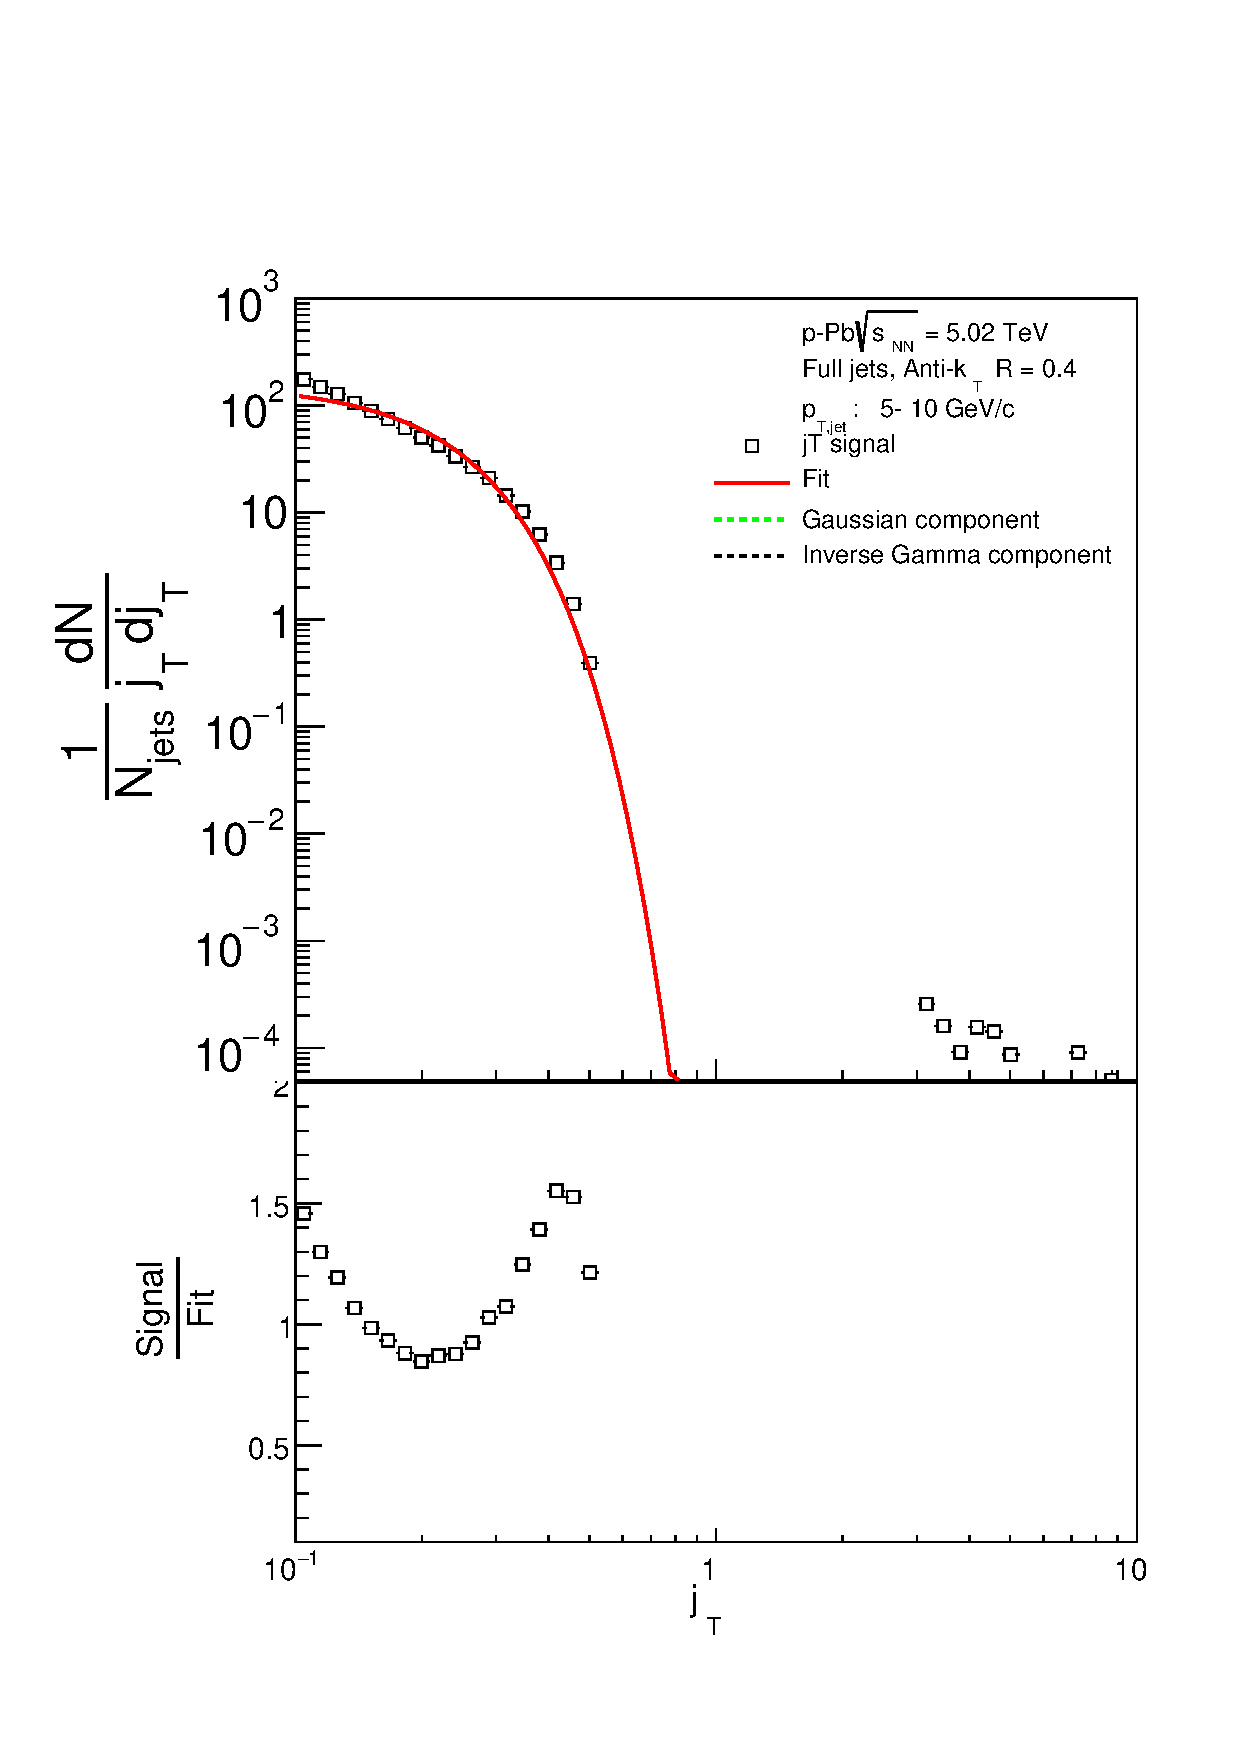
\includegraphics[width=0.95\textwidth]{RooUnfold/figs/JetConejTSignalFit/JetConejTSignalFitNFin00JetPt00randomBgBayes}
%\end{subfigure}
%\begin{subfigure}{0.24\textwidth}
%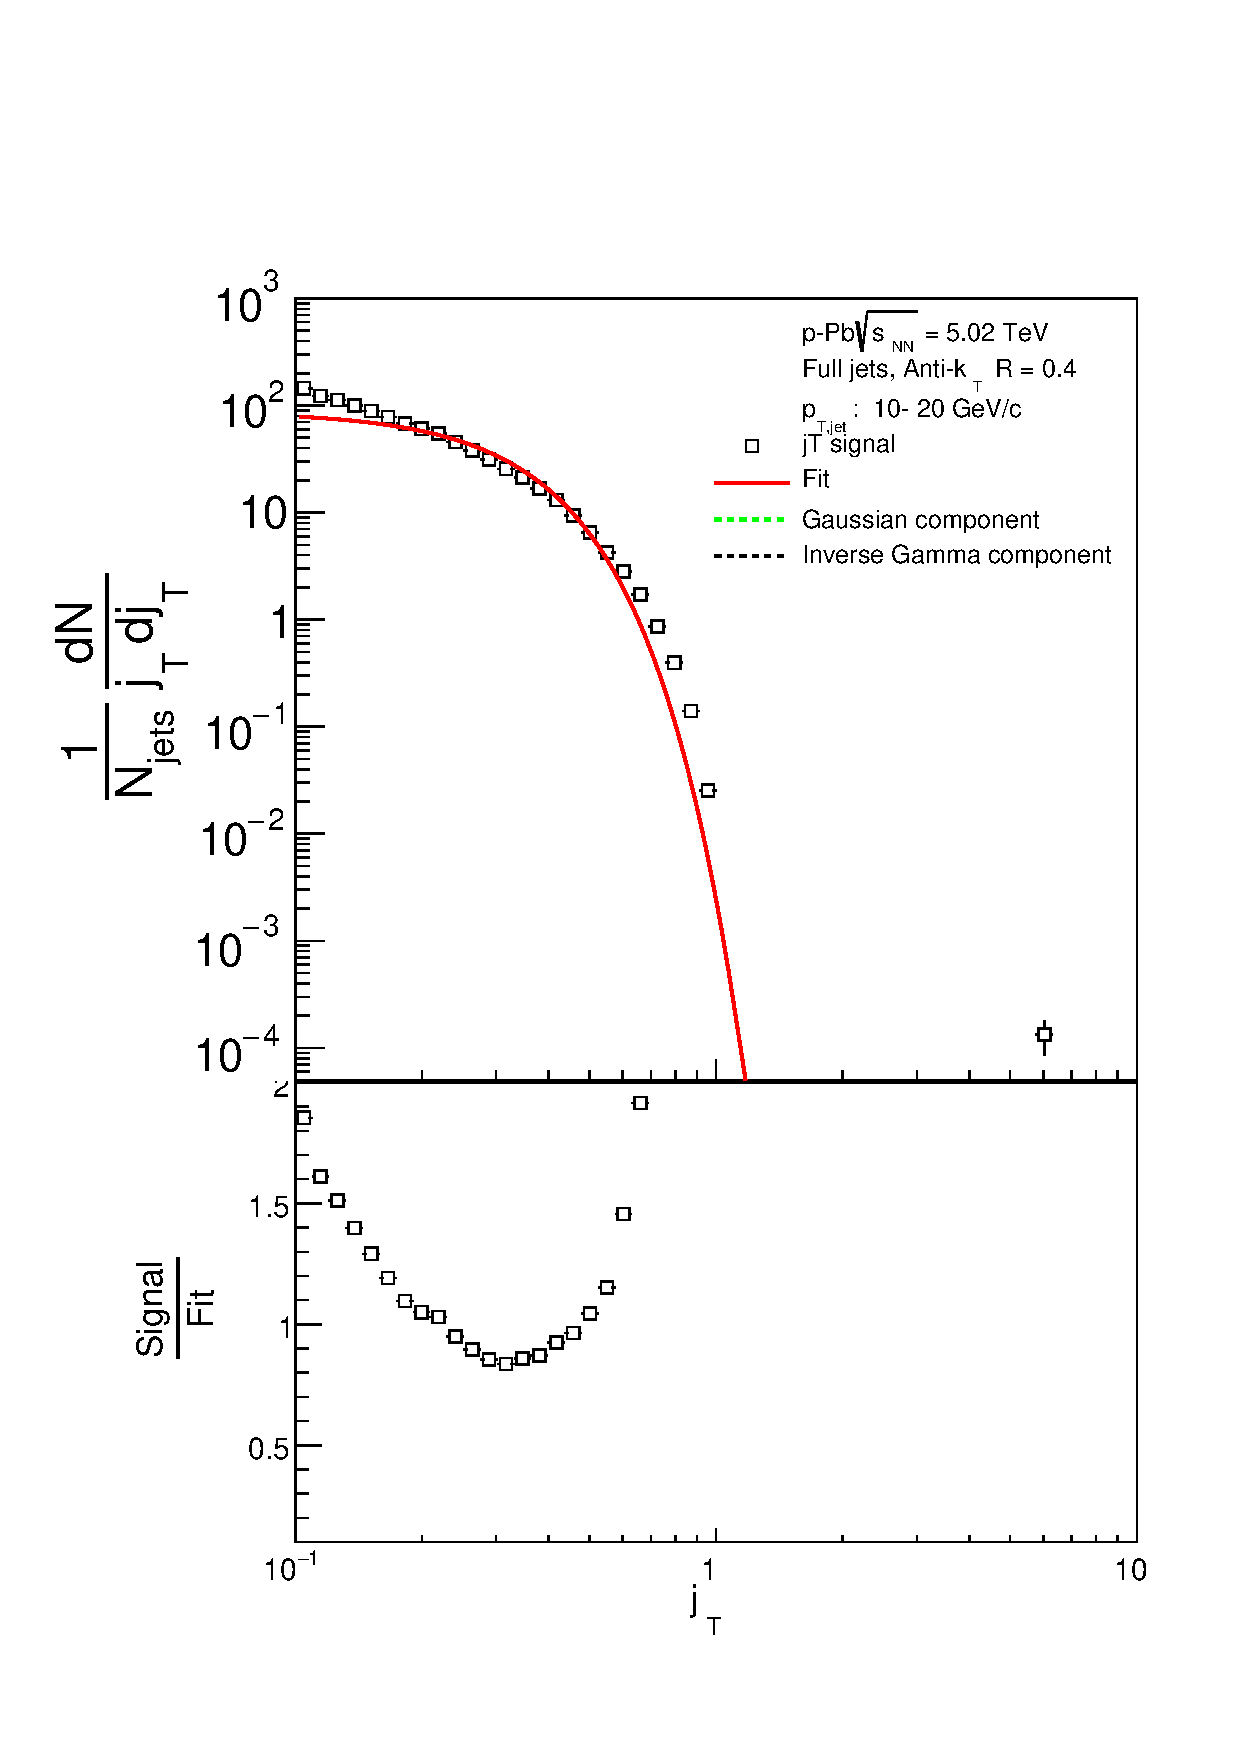
\includegraphics[width=0.95\textwidth]{RooUnfold/figs/JetConejTSignalFit/JetConejTSignalFitNFin00JetPt01randomBgBayes}
%\end{subfigure}
%\begin{subfigure}{0.24\textwidth}
%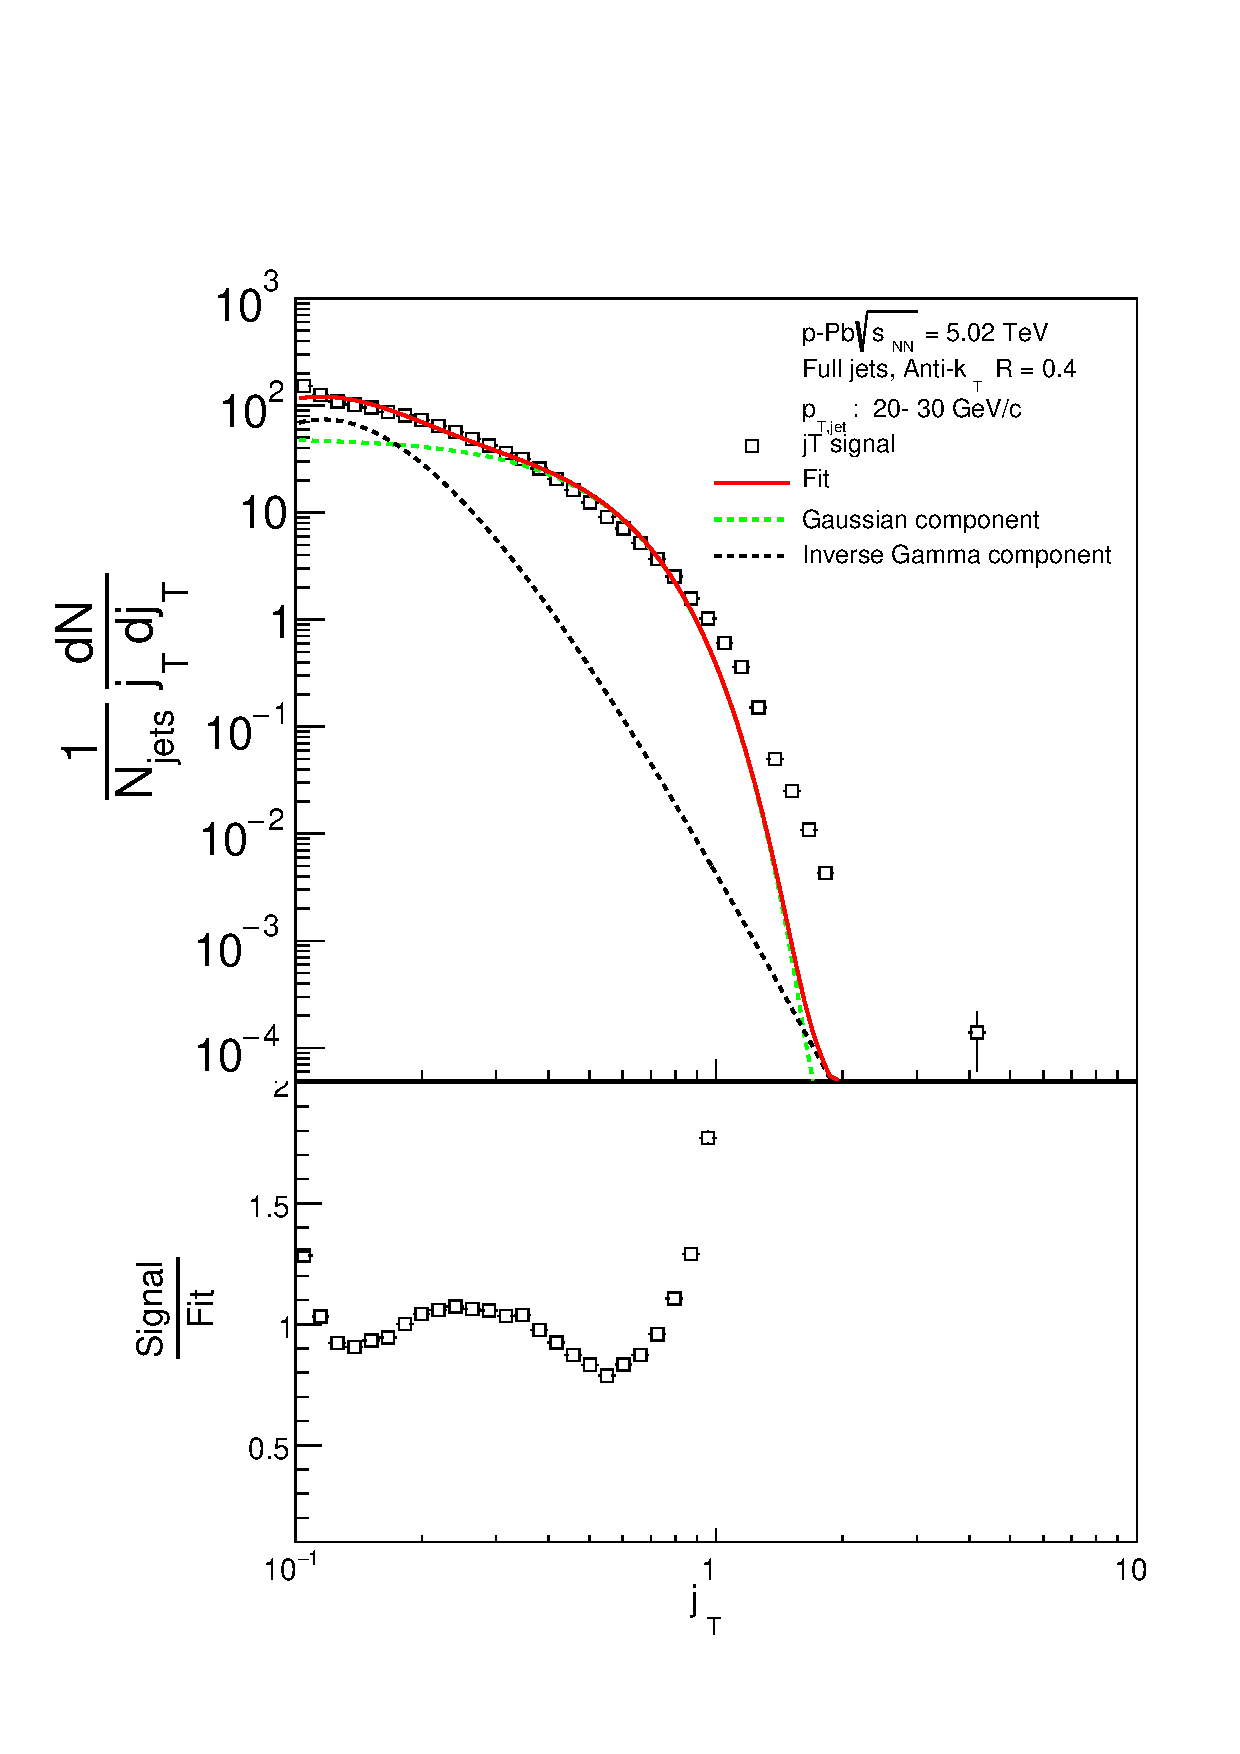
\includegraphics[width=0.95\textwidth]{RooUnfold/figs/JetConejTSignalFit/JetConejTSignalFitNFin00JetPt02randomBgBayes}
%\end{subfigure}
%\begin{subfigure}{0.24\textwidth}
%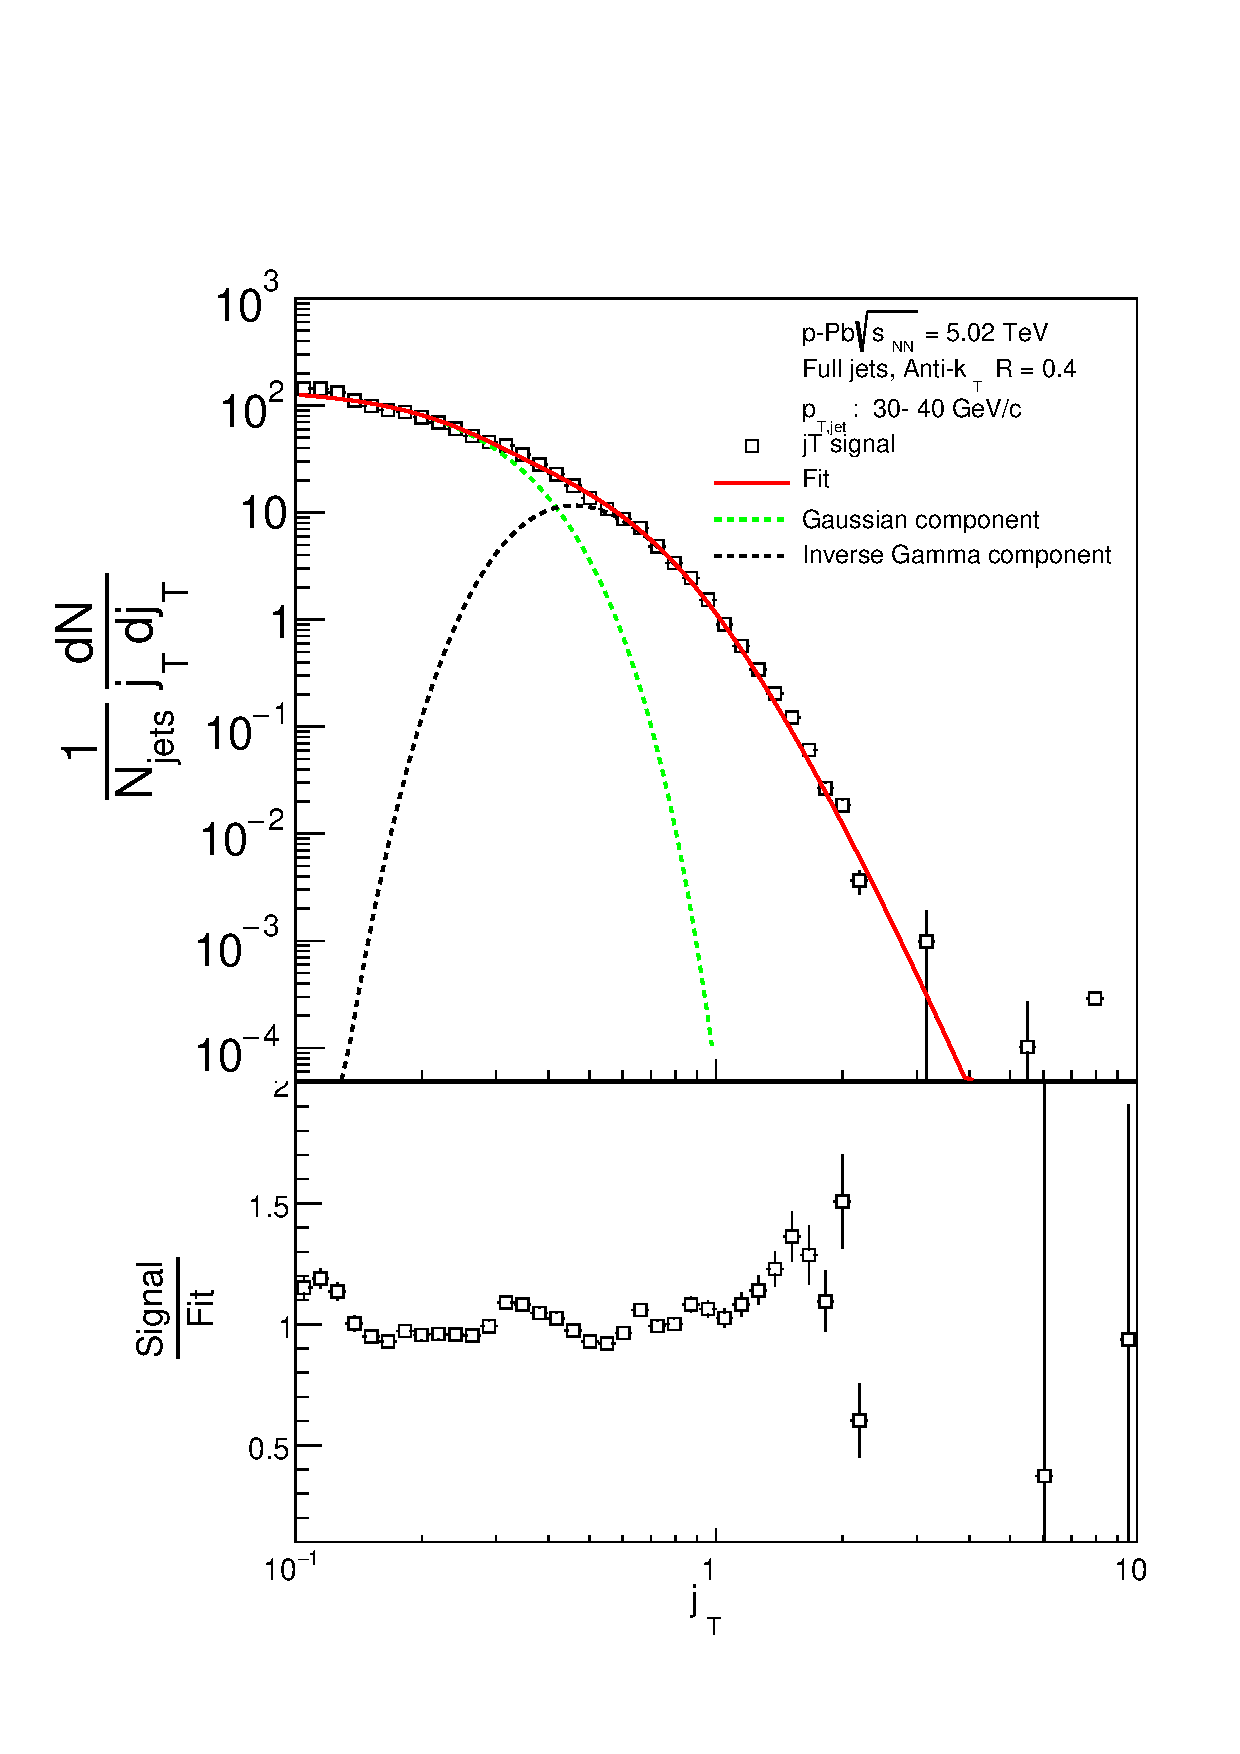
\includegraphics[width=0.95\textwidth]{RooUnfold/figs/JetConejTSignalFit/JetConejTSignalFitNFin00JetPt03randomBgBayes}
%\end{subfigure}
\begin{subfigure}{0.24\textwidth}
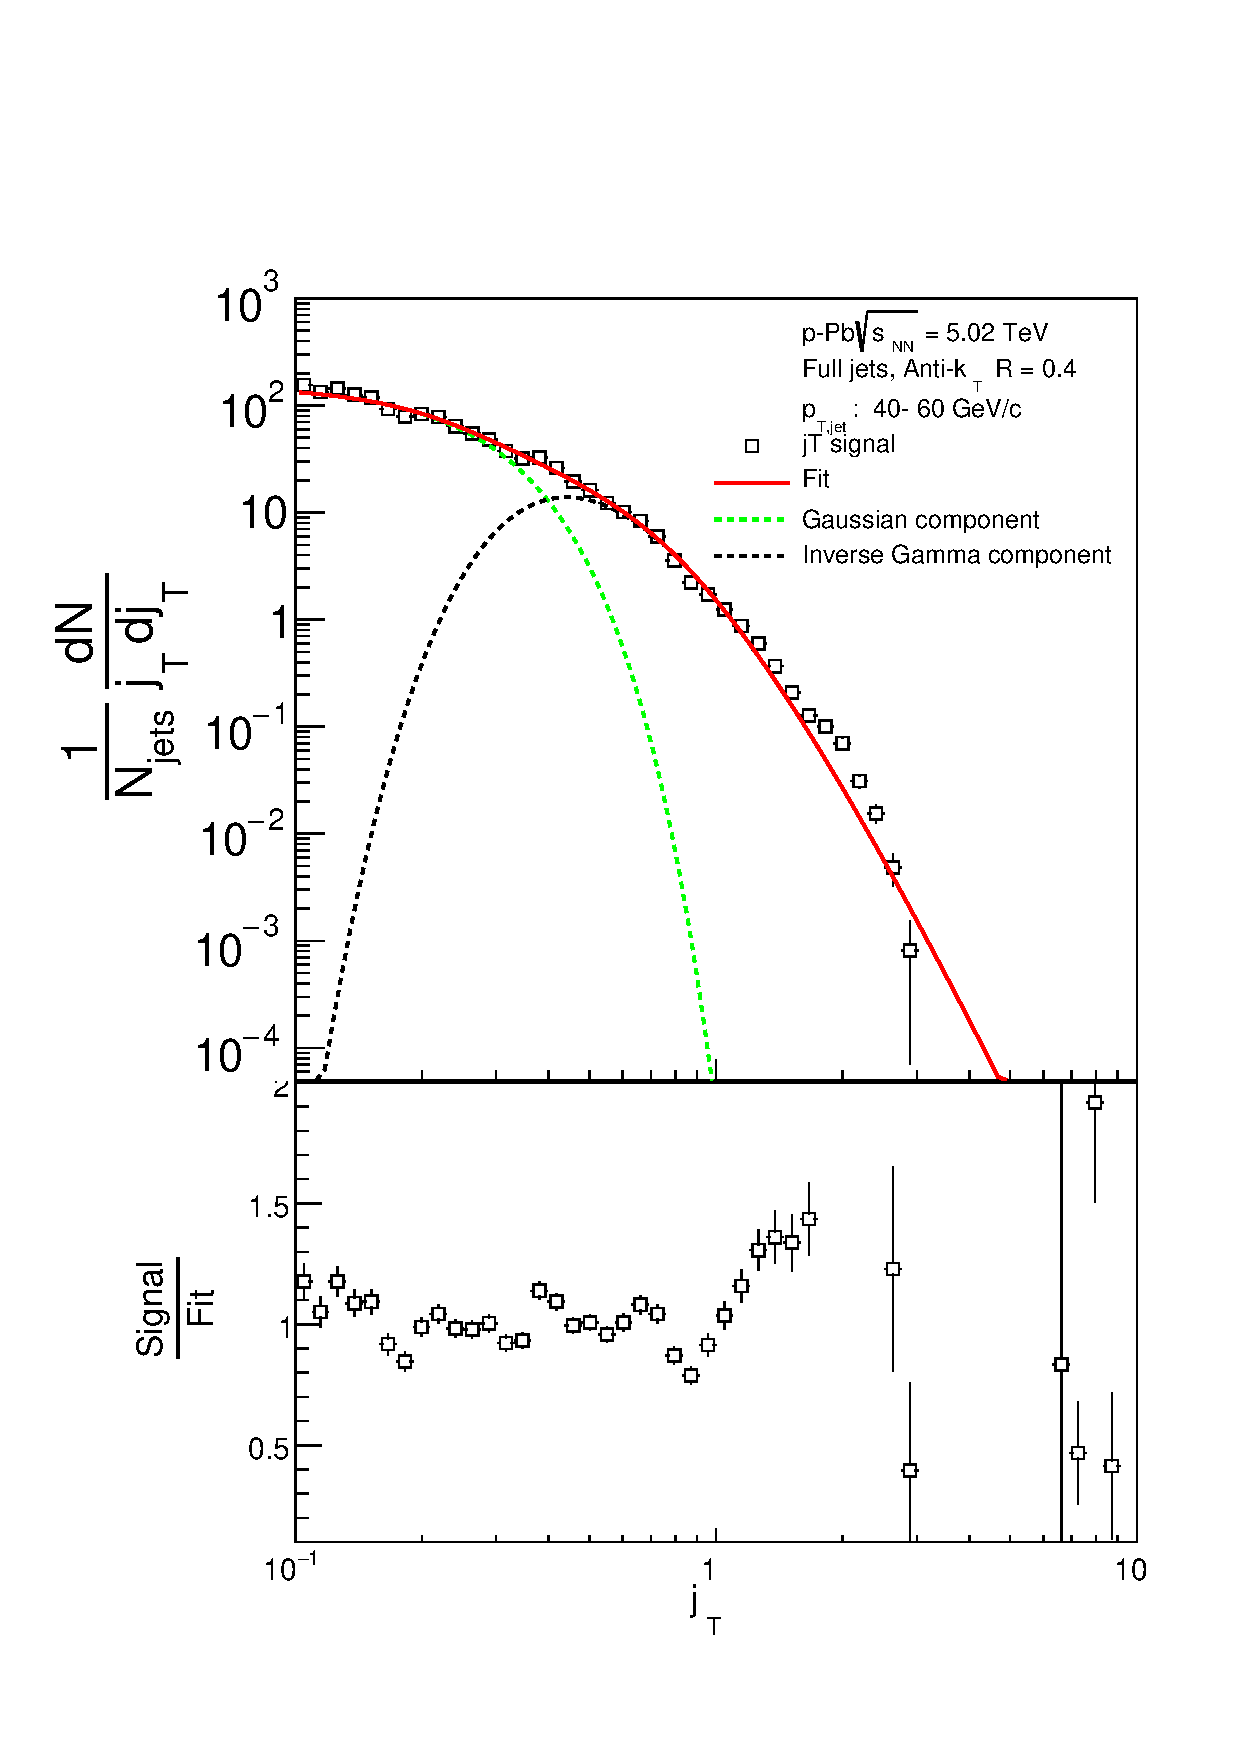
\includegraphics[width=0.95\textwidth]{results/JetConejTSignalFit/JetConejTSignalFitNFin00JetPt04randomBgBayes}
\end{subfigure}
\begin{subfigure}{0.24\textwidth}
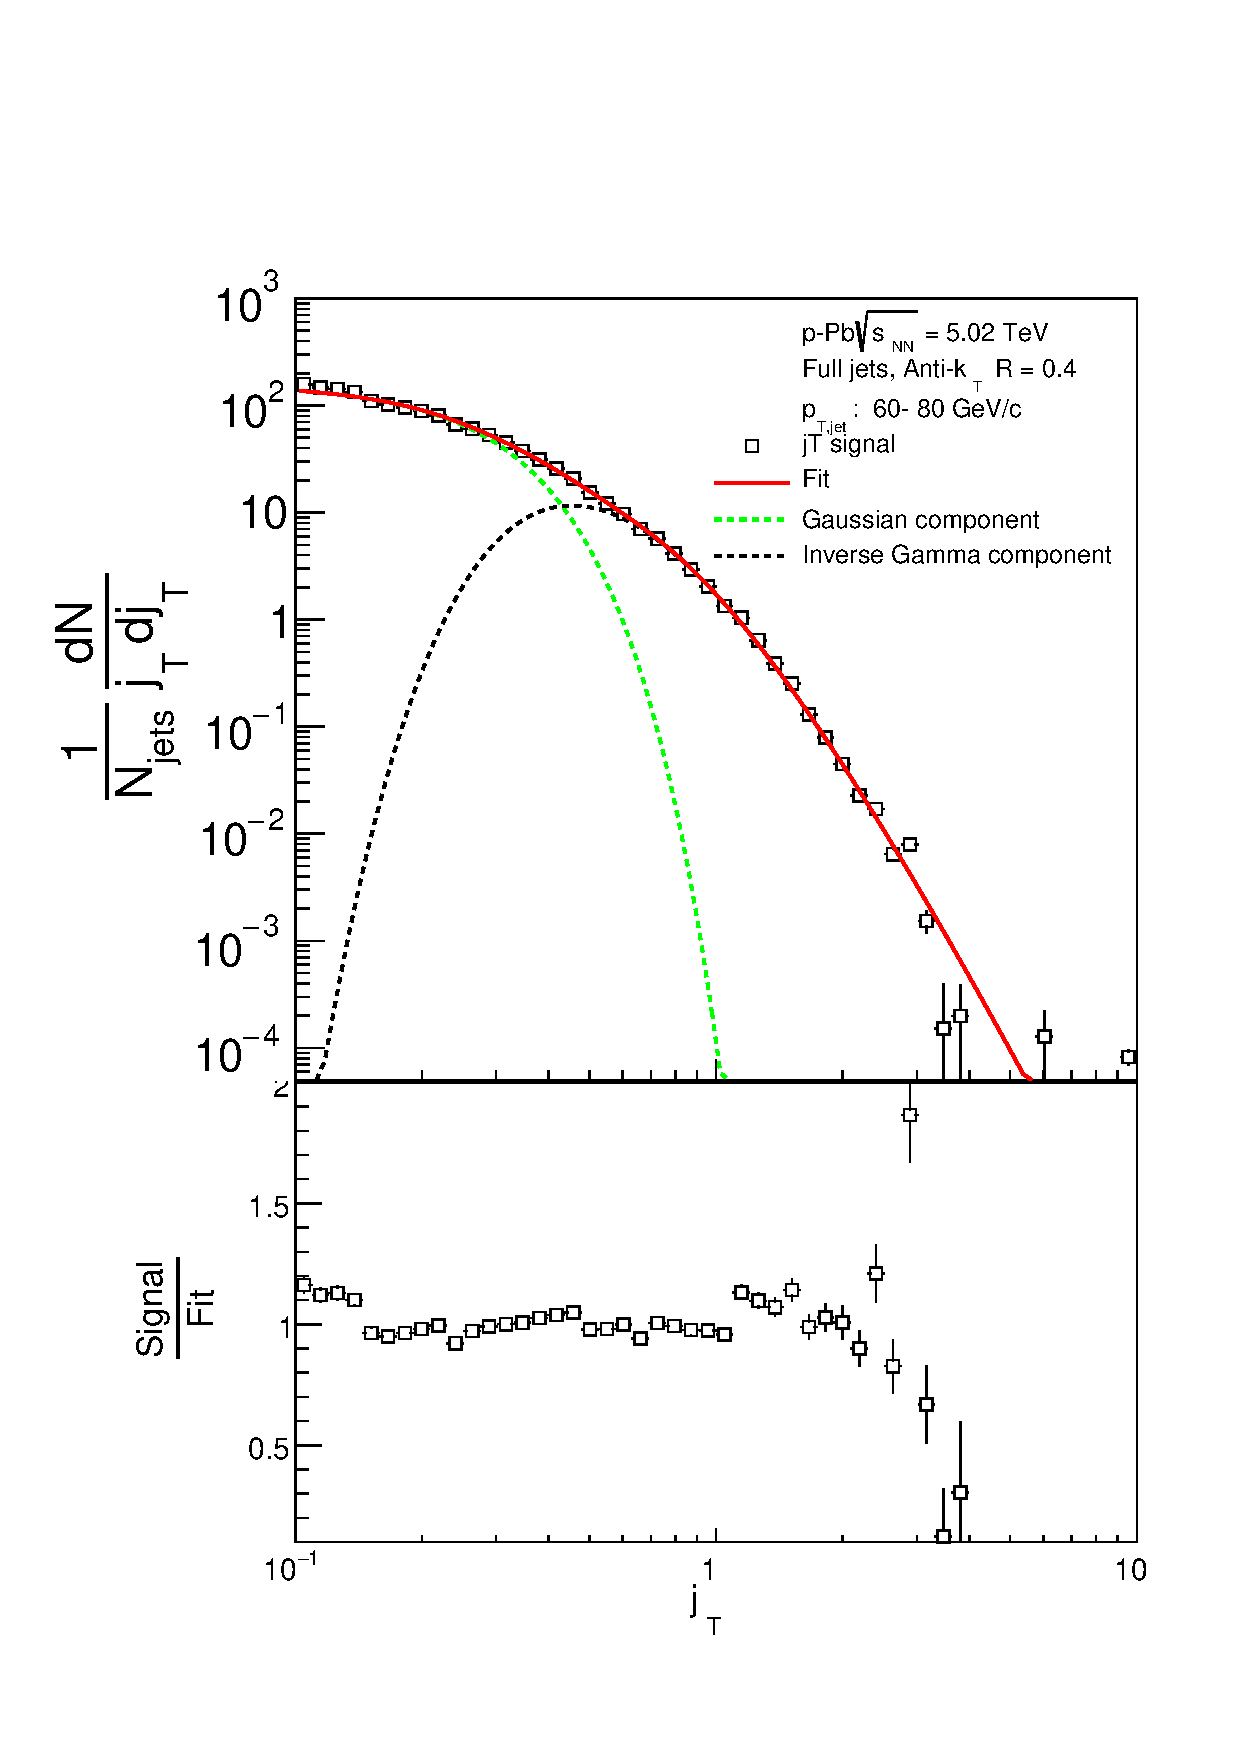
\includegraphics[width=0.95\textwidth]{results/JetConejTSignalFit/JetConejTSignalFitNFin00JetPt05randomBgBayes}
\end{subfigure}
\begin{subfigure}{0.24\textwidth}
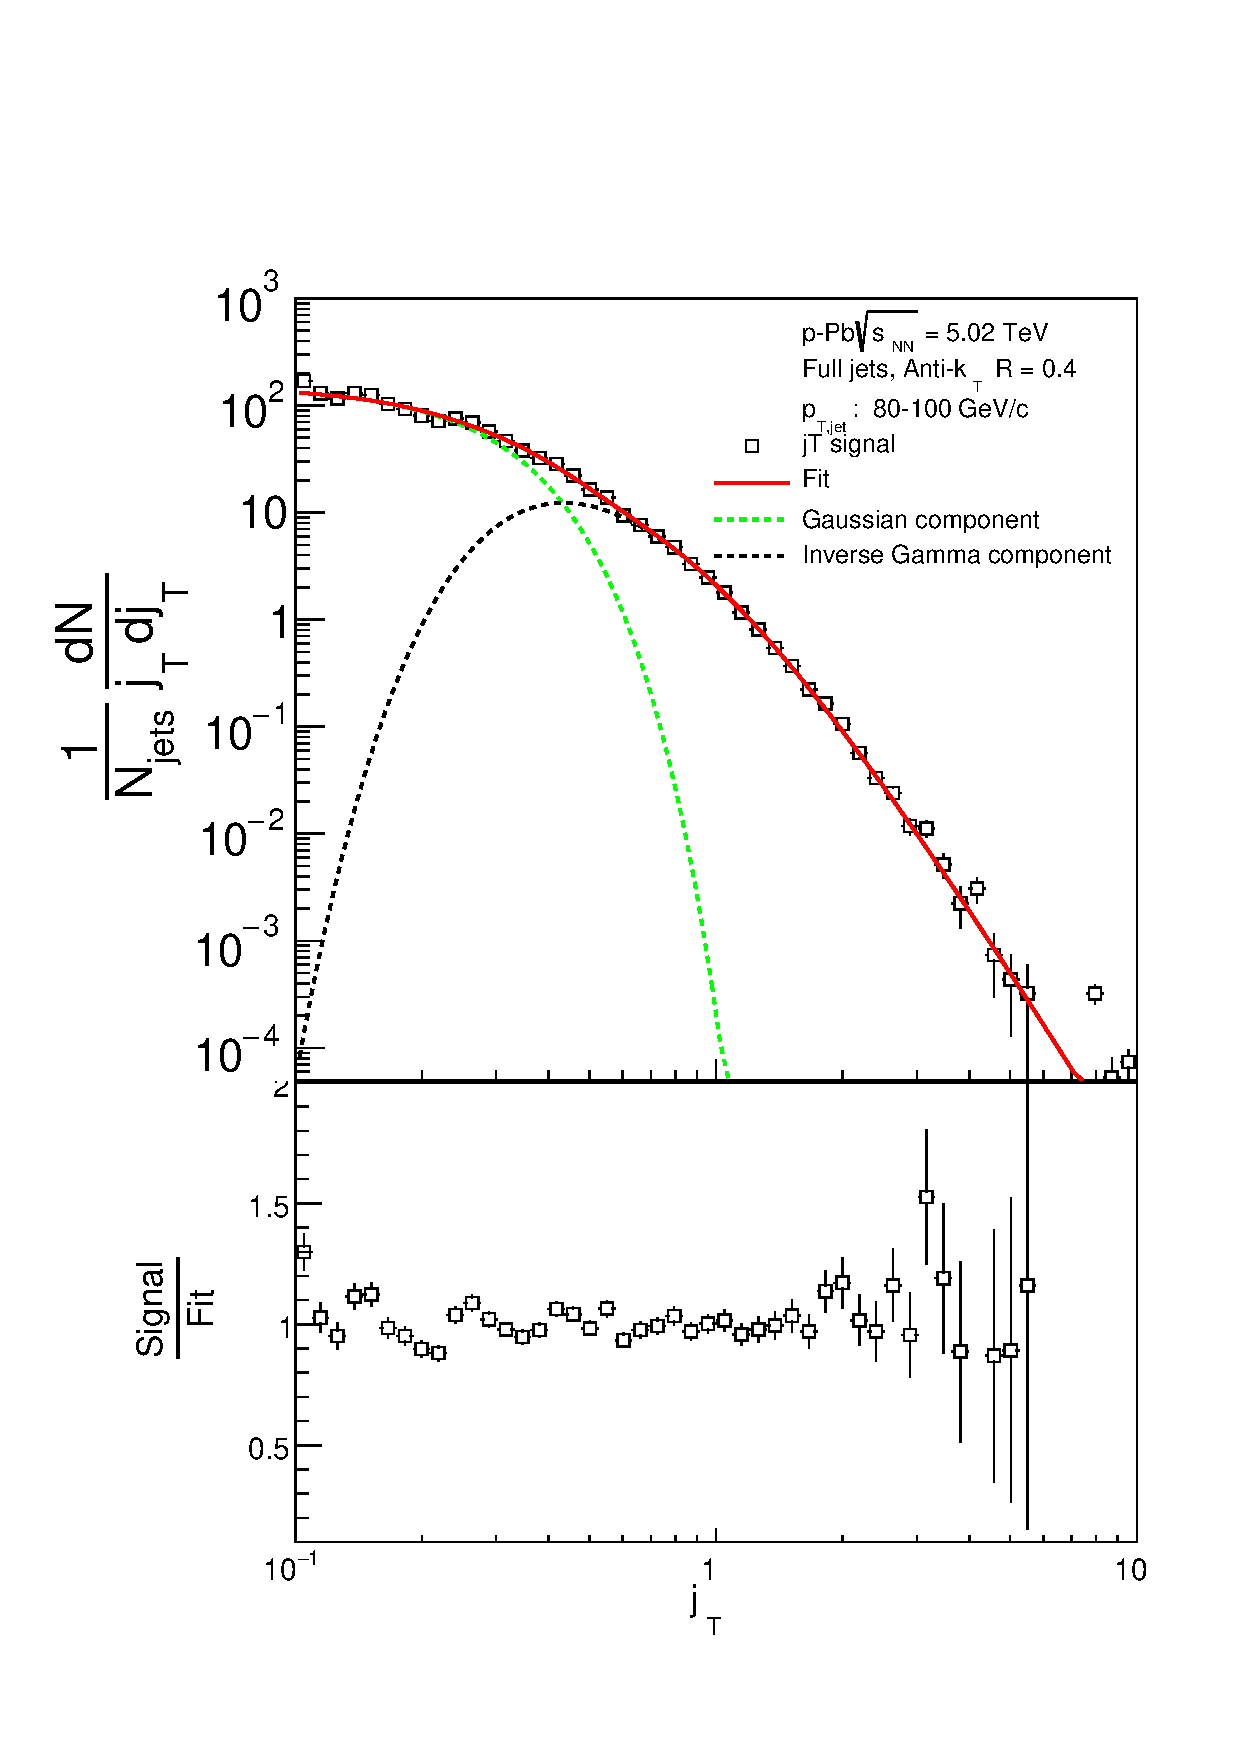
\includegraphics[width=0.95\textwidth]{results/JetConejTSignalFit/JetConejTSignalFitNFin00JetPt06randomBgBayes}
\end{subfigure}
\begin{subfigure}{0.24\textwidth}
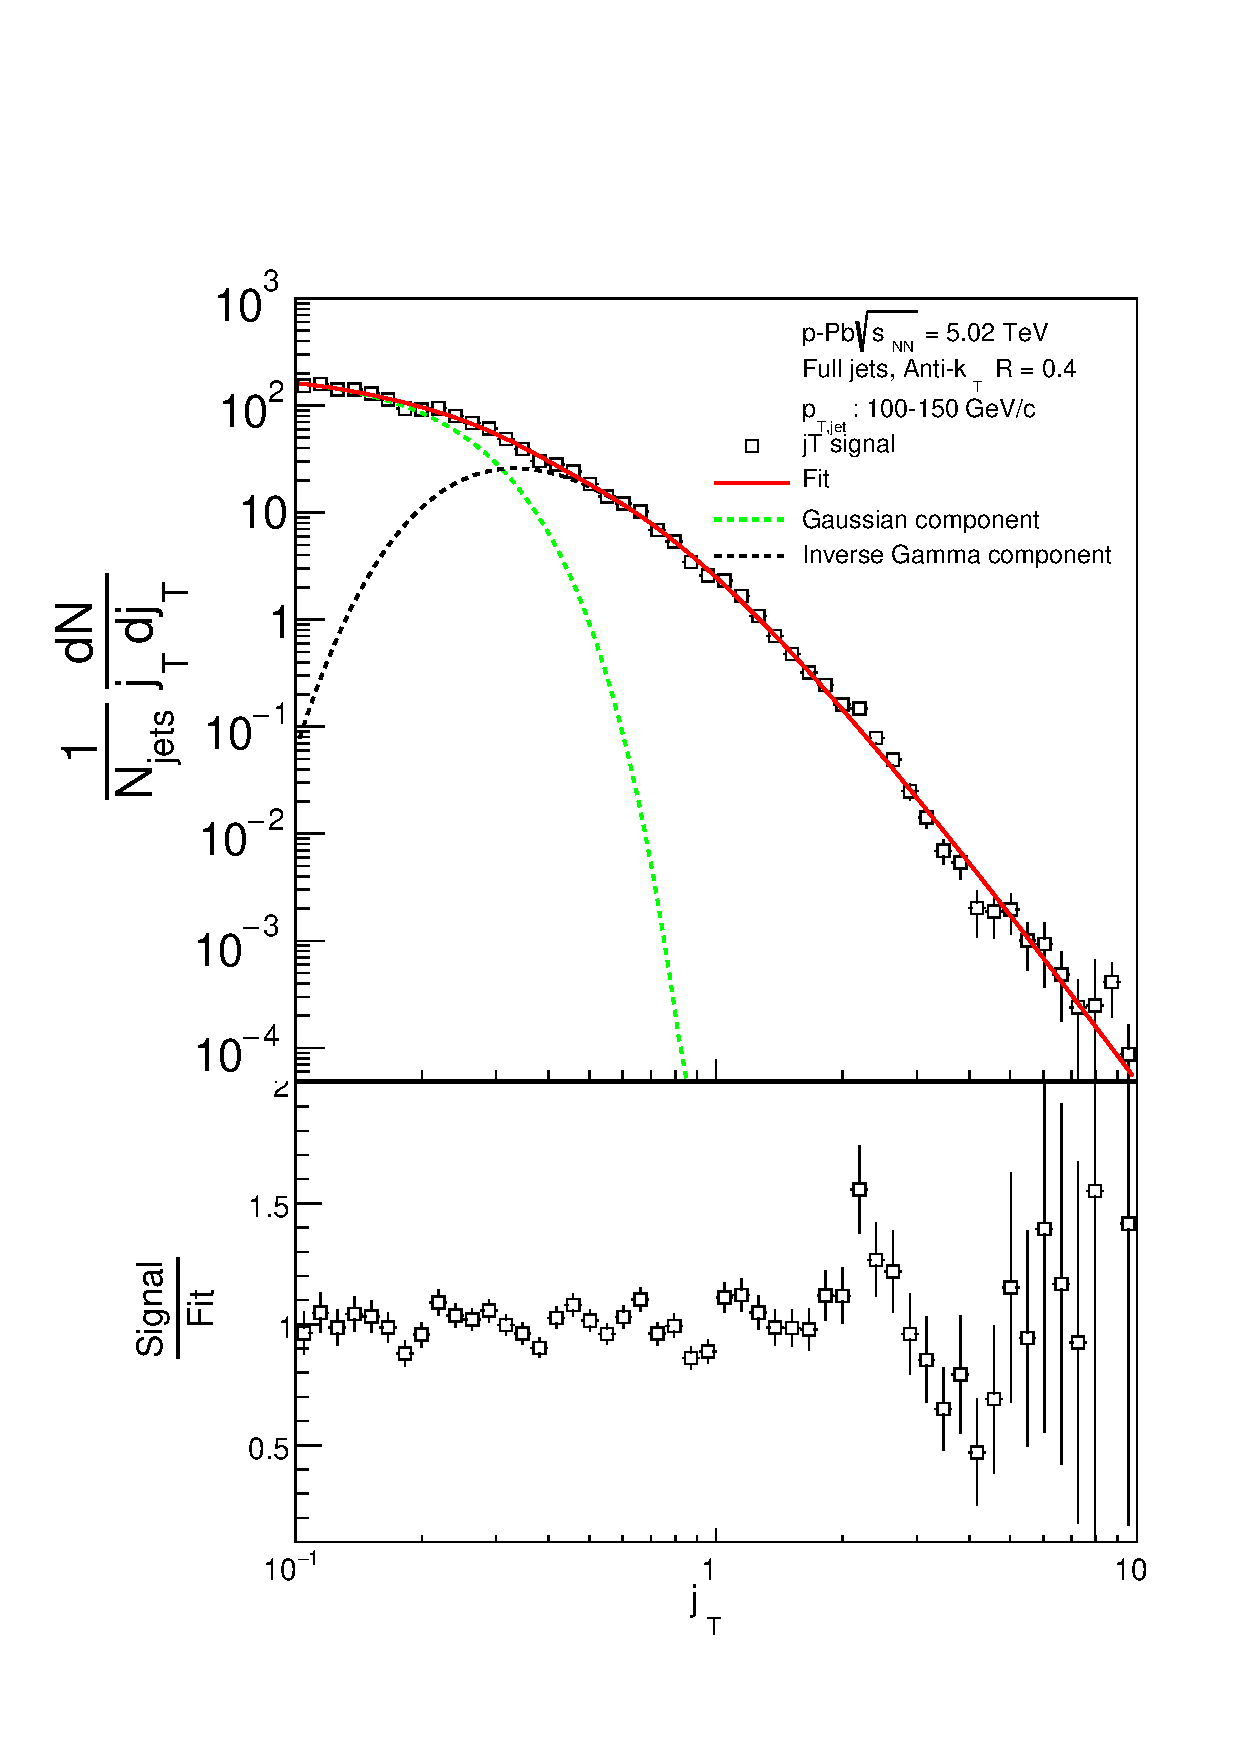
\includegraphics[width=0.95\textwidth]{results/JetConejTSignalFit/JetConejTSignalFitNFin00JetPt07randomBgBayes}
\end{subfigure}
\caption{$j_T$ signal with random bacgkround subtraction fits in different jet $p_T$ bins}
\label{fig:fitsrandombg}
\end{figure}

\begin{figure}
\centering
\begin{subfigure}{0.24\textwidth}
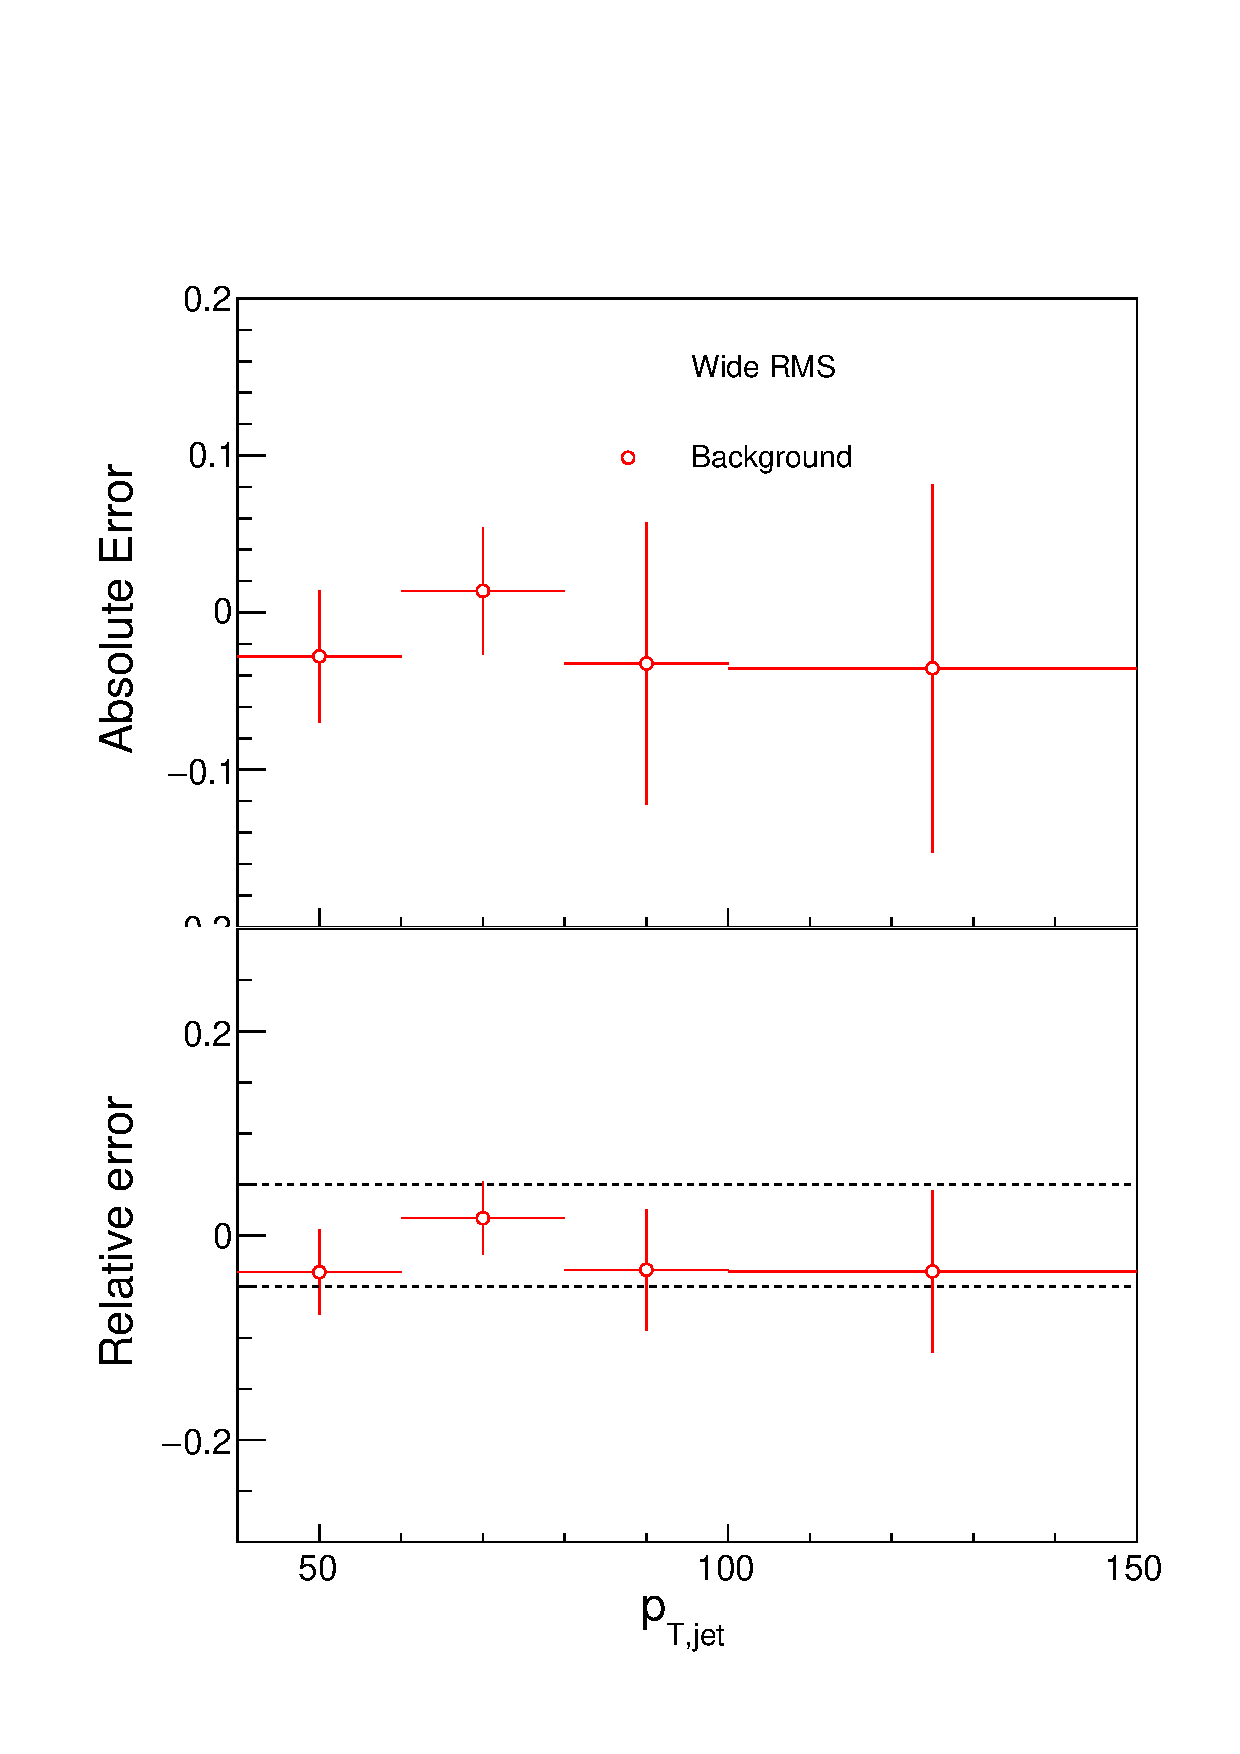
\includegraphics[width=0.95\textwidth]{results/SystematicErrors/SystematicErrorsGammaRMS_BgNFin00JetPt08_linx_data}
\end{subfigure}
\begin{subfigure}{0.24\textwidth}
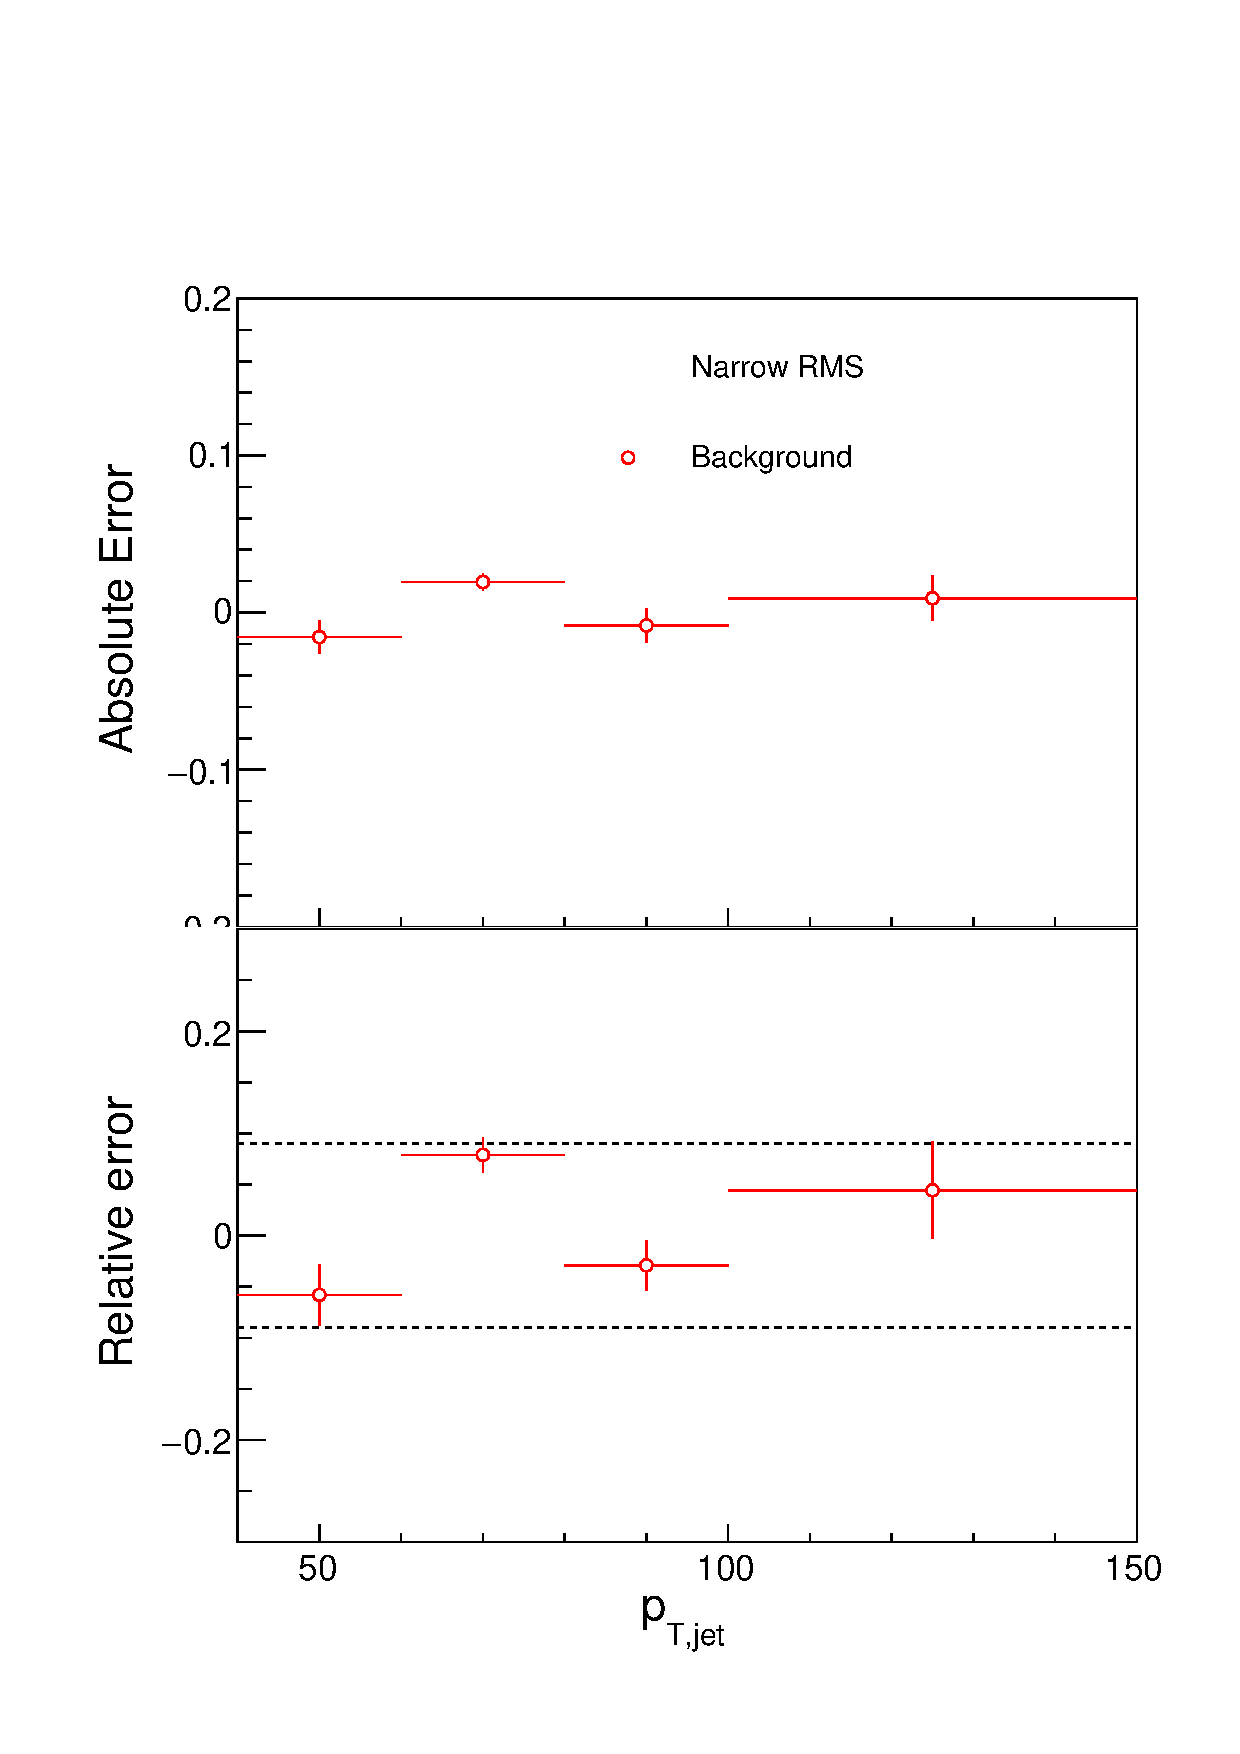
\includegraphics[width=0.95\textwidth]{results/SystematicErrors/SystematicErrorsGausRMS_BgNFin00JetPt08_linx_data}
\end{subfigure}
\caption{Differences between perpendicular cone and random background subtraction in the resulting RMS values.}
\label{fig:systbg}
\end{figure}

\begin{figure}
\centering
%\begin{subfigure}{0.24\textwidth}
%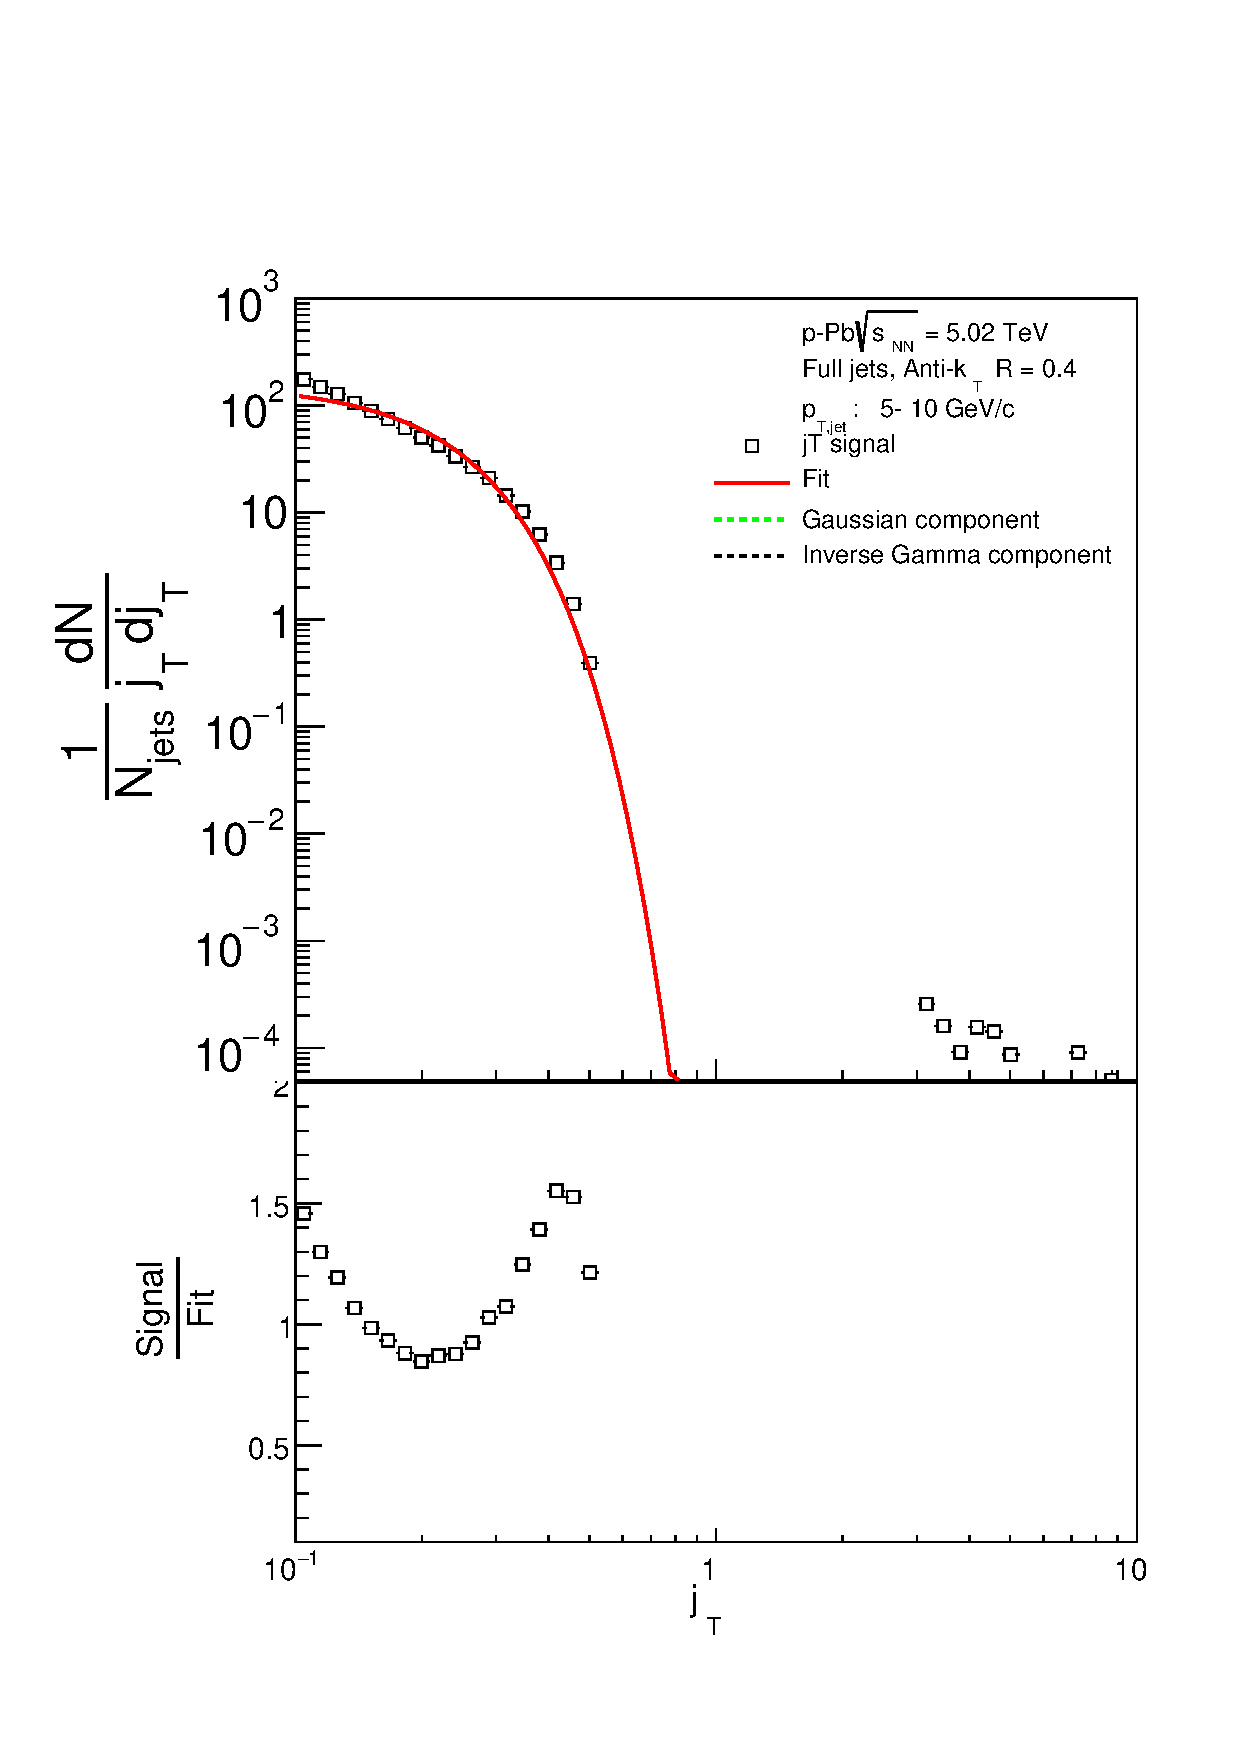
\includegraphics[width=0.95\textwidth]{RooUnfold/figs/JetConejTSignalFit/JetConejTSignalFitNFin00JetPt00randomBgBayes}
%\end{subfigure}
%\begin{subfigure}{0.24\textwidth}
%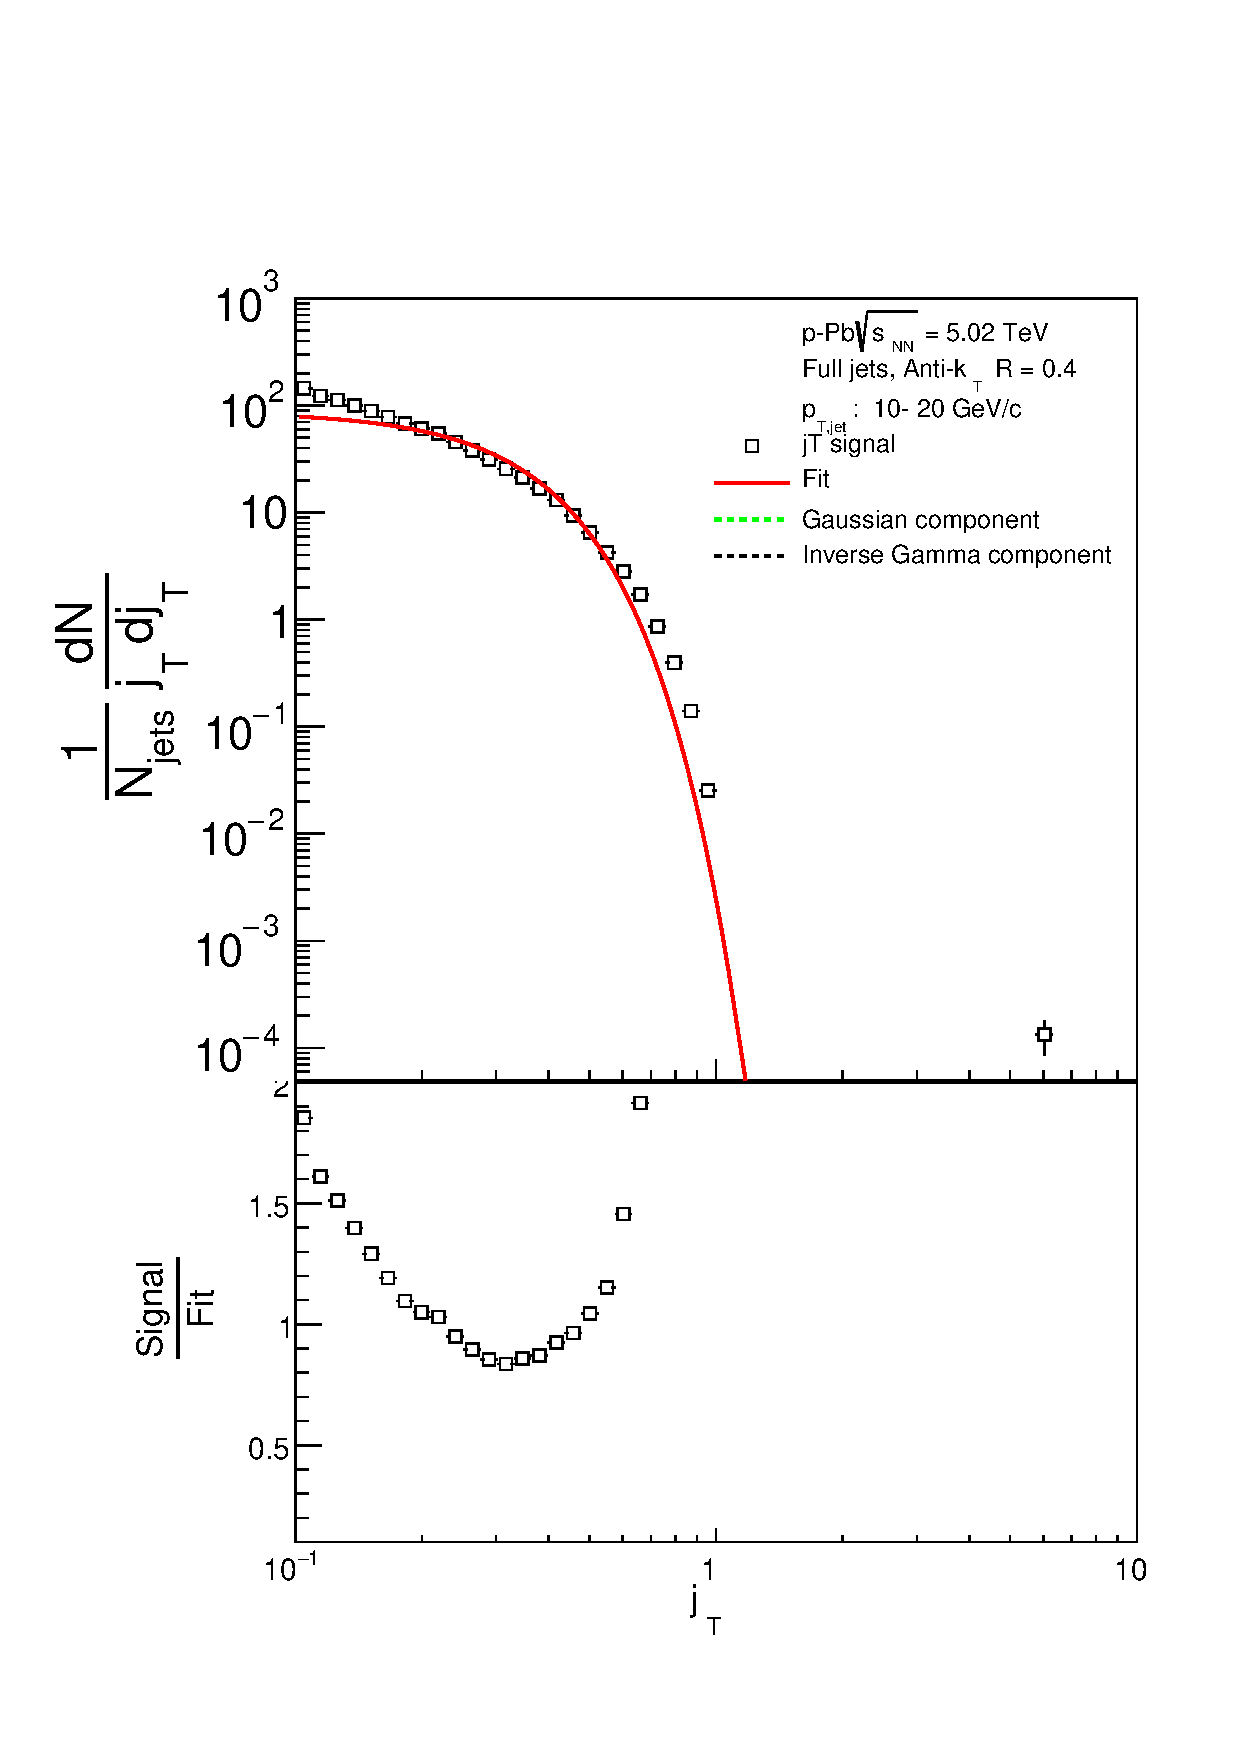
\includegraphics[width=0.95\textwidth]{RooUnfold/figs/JetConejTSignalFit/JetConejTSignalFitNFin00JetPt01randomBgBayes}
%\end{subfigure}
%\begin{subfigure}{0.24\textwidth}
%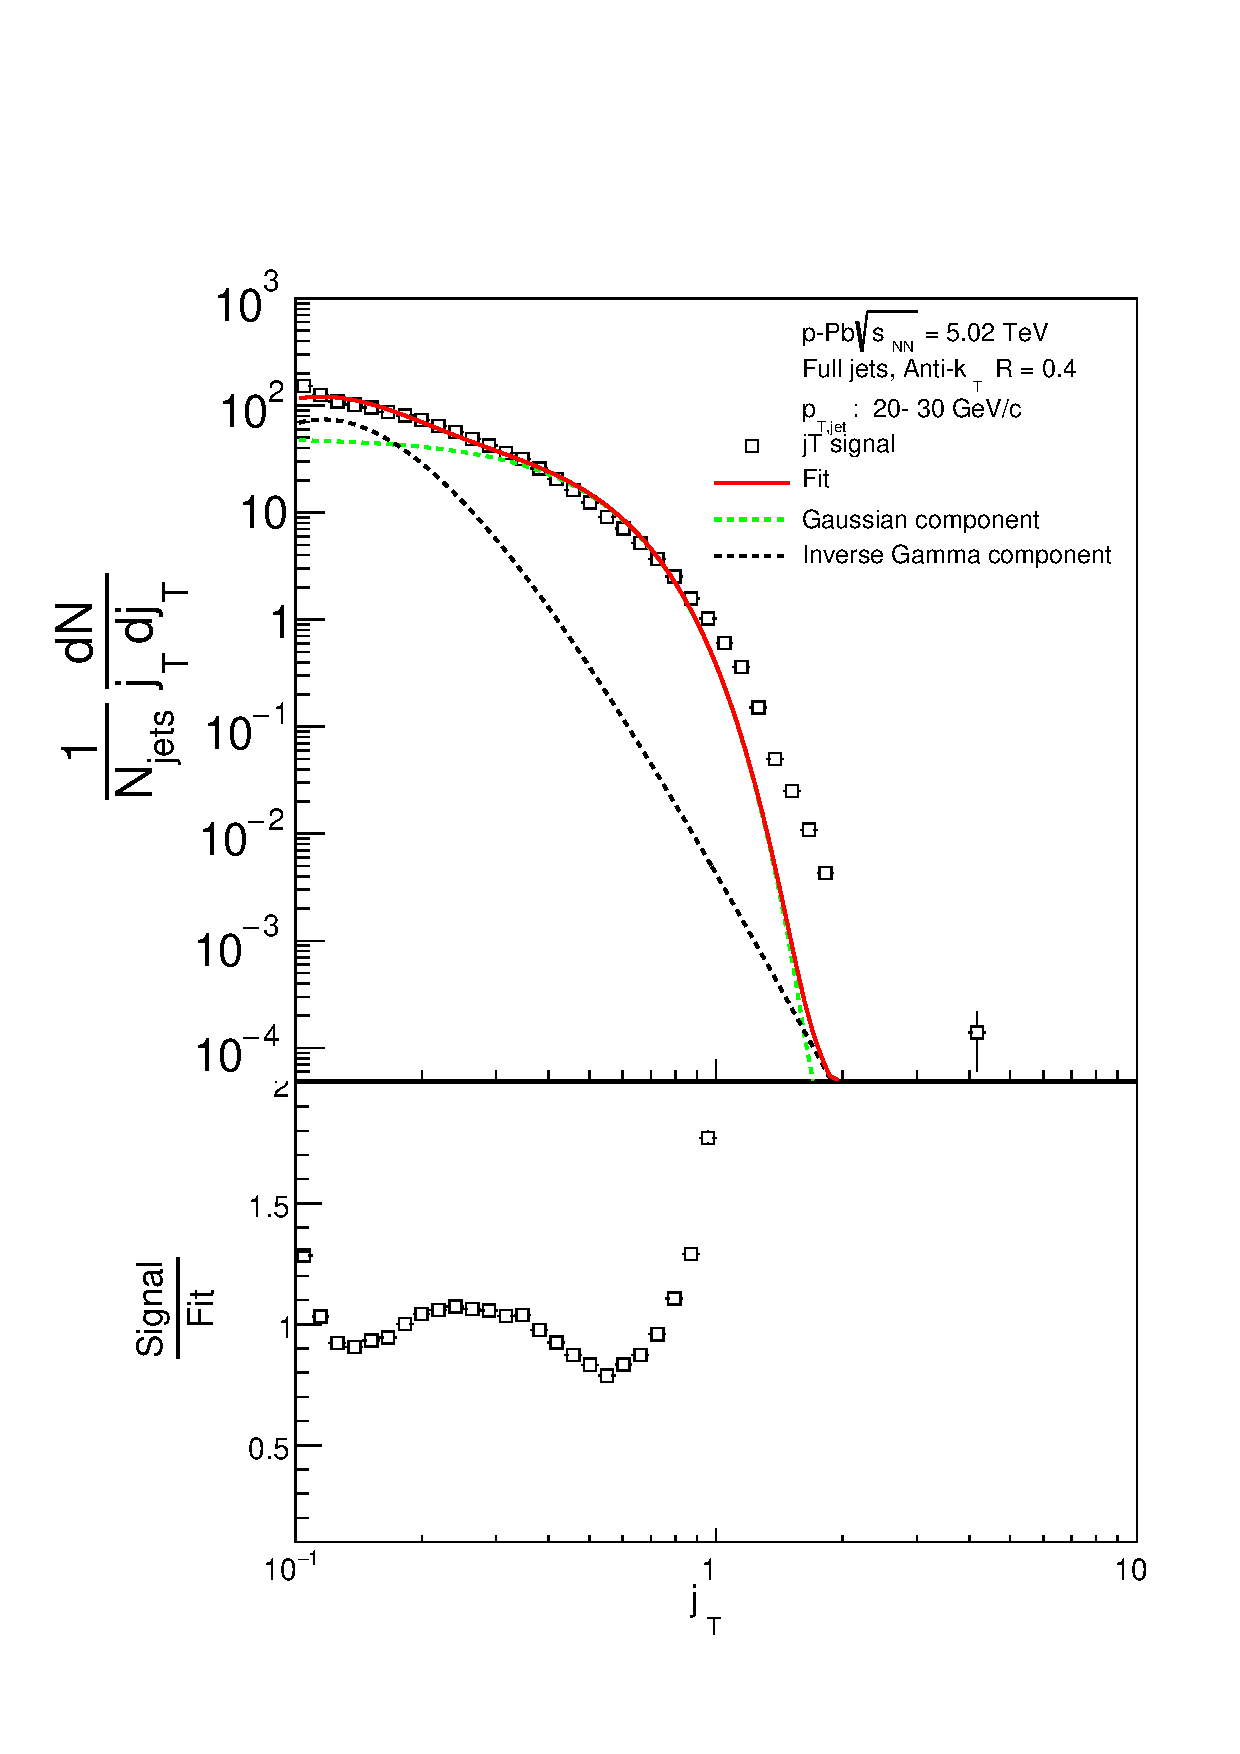
\includegraphics[width=0.95\textwidth]{RooUnfold/figs/JetConejTSignalFit/JetConejTSignalFitNFin00JetPt02randomBgBayes}
%\end{subfigure}
%\begin{subfigure}{0.24\textwidth}
%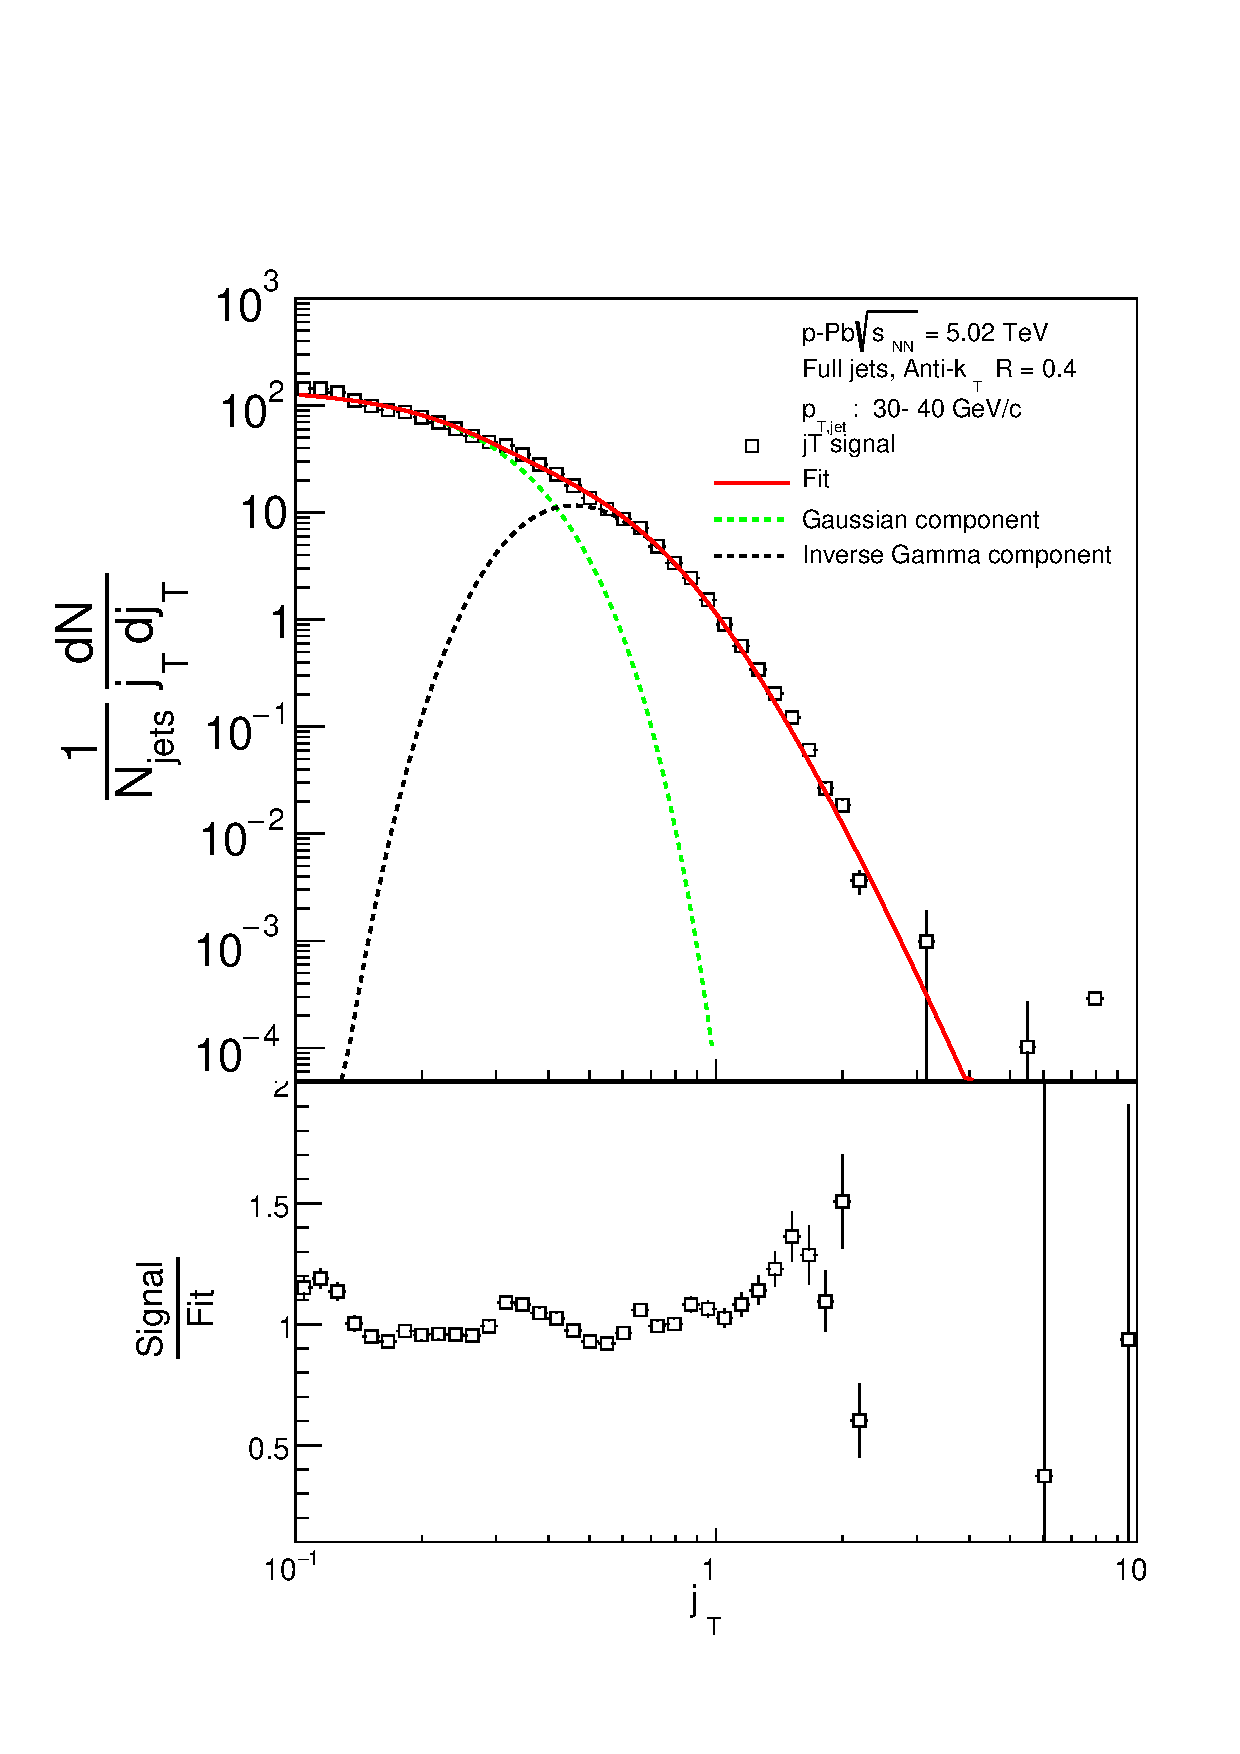
\includegraphics[width=0.95\textwidth]{RooUnfold/figs/JetConejTSignalFit/JetConejTSignalFitNFin00JetPt03randomBgBayes}
%\end{subfigure}
\begin{subfigure}{0.24\textwidth}
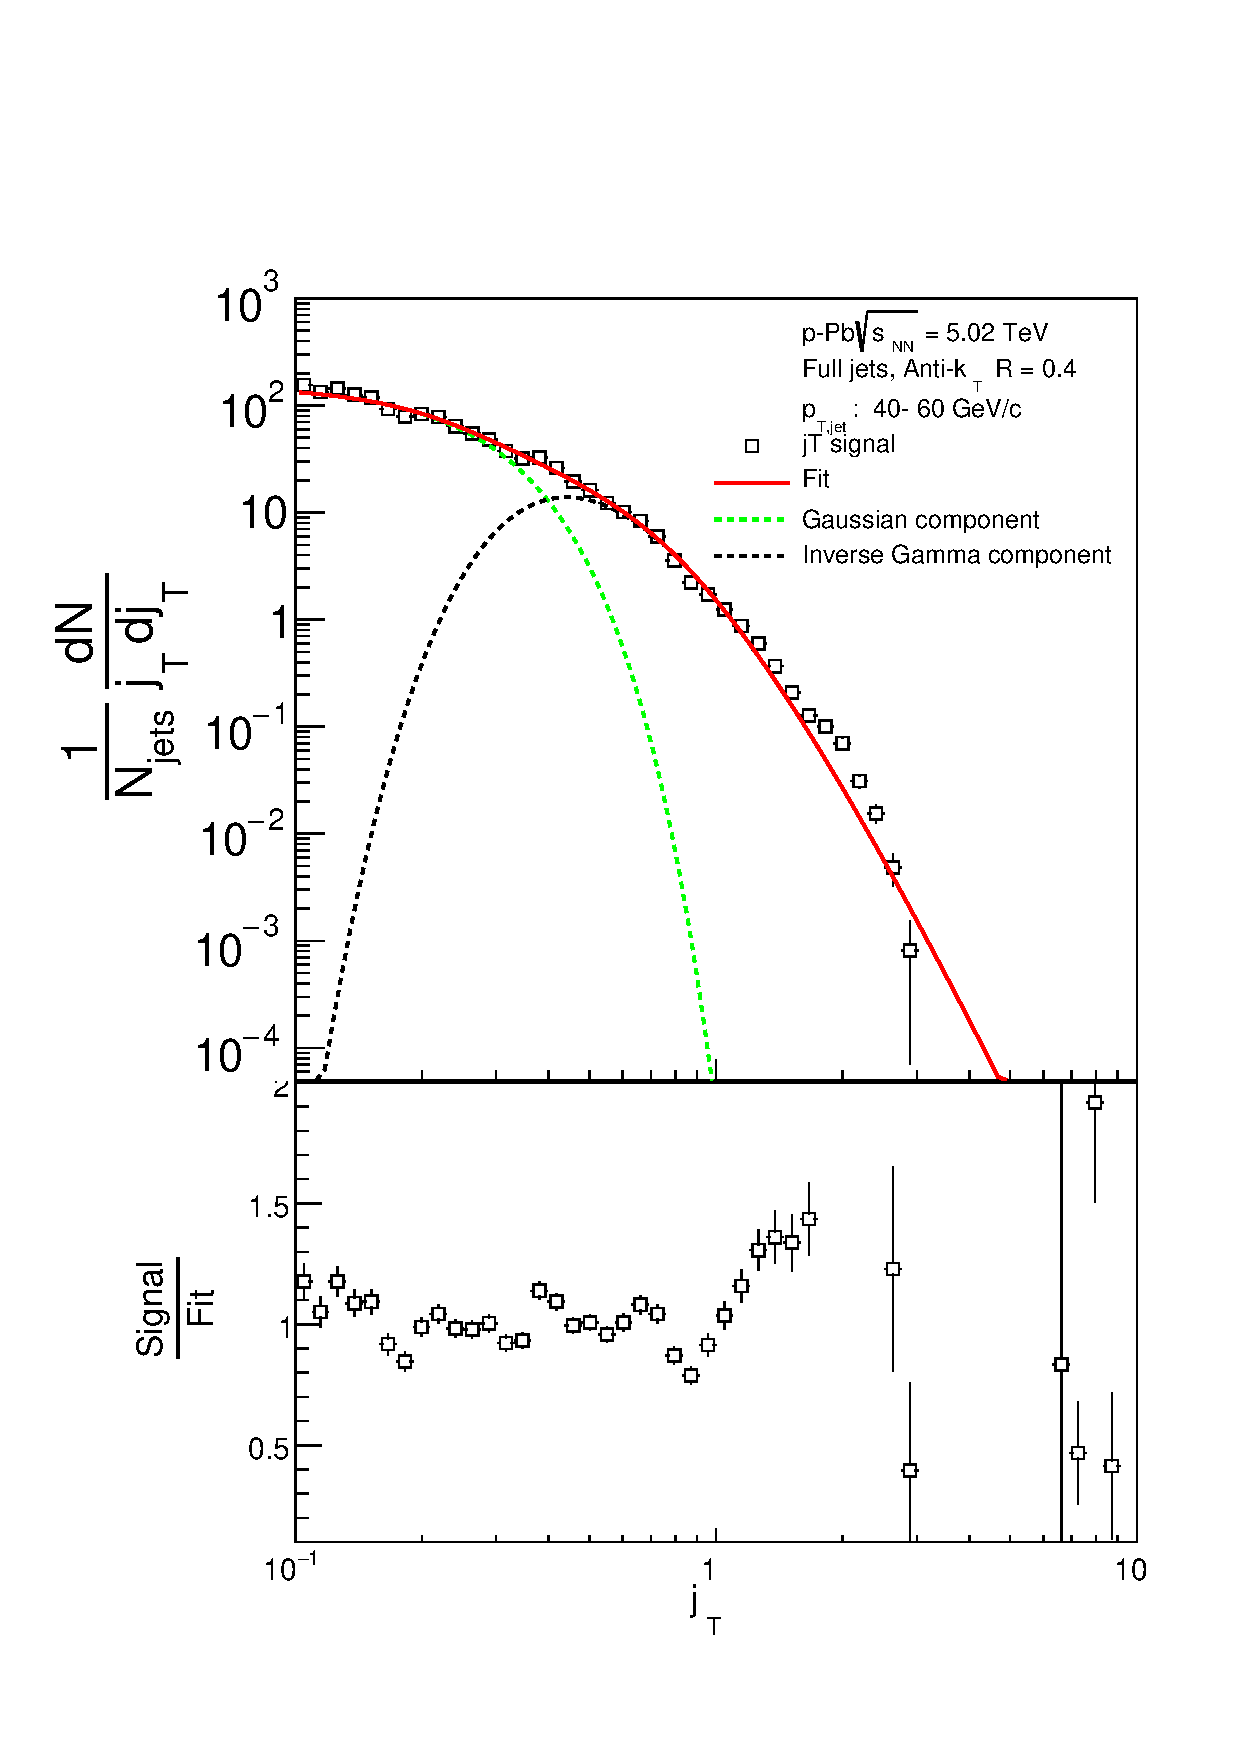
\includegraphics[width=0.95\textwidth]{results/JetConejTSignalFit/JetConejTSignalFitNFin00JetPt04randomBgBayes}
\end{subfigure}
\begin{subfigure}{0.24\textwidth}
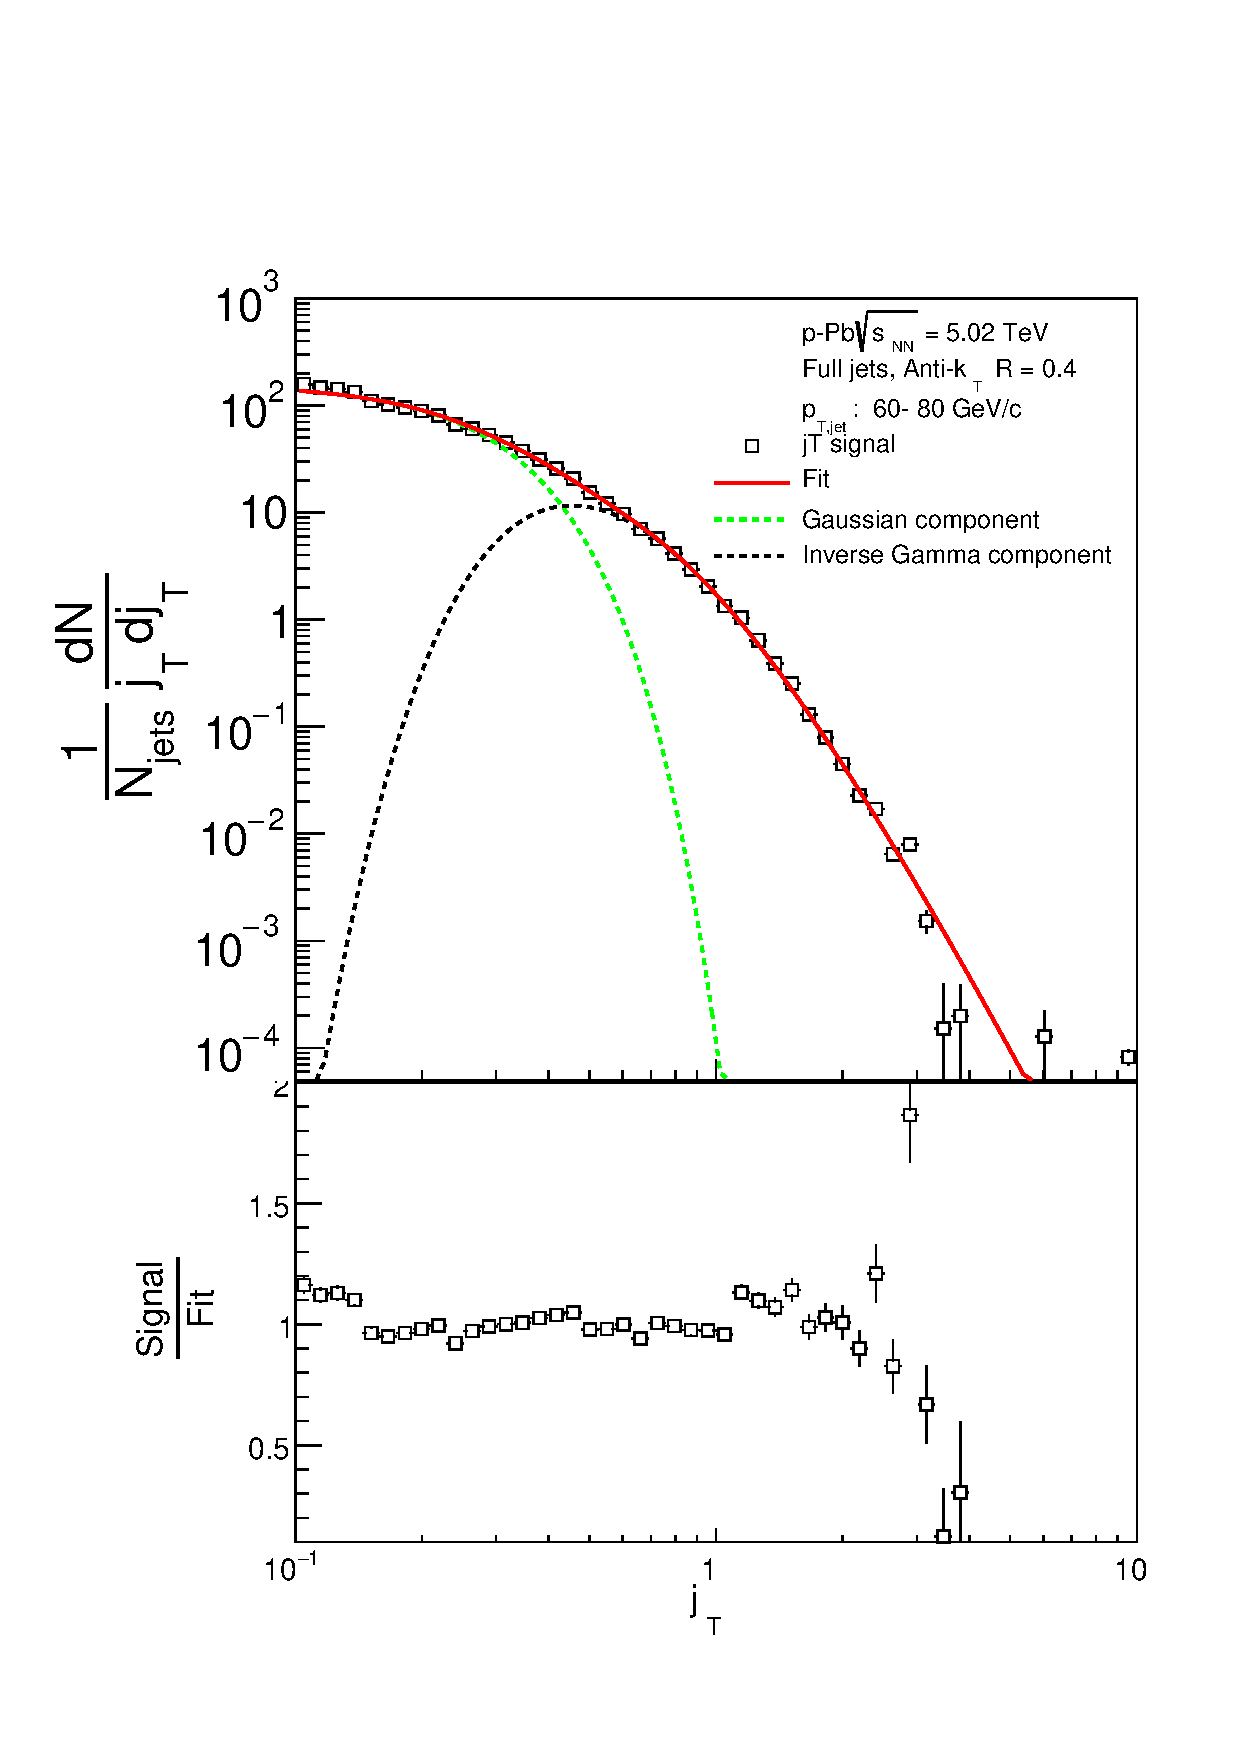
\includegraphics[width=0.95\textwidth]{results/JetConejTSignalFit/JetConejTSignalFitNFin00JetPt05randomBgBayes}
\end{subfigure}
\begin{subfigure}{0.24\textwidth}
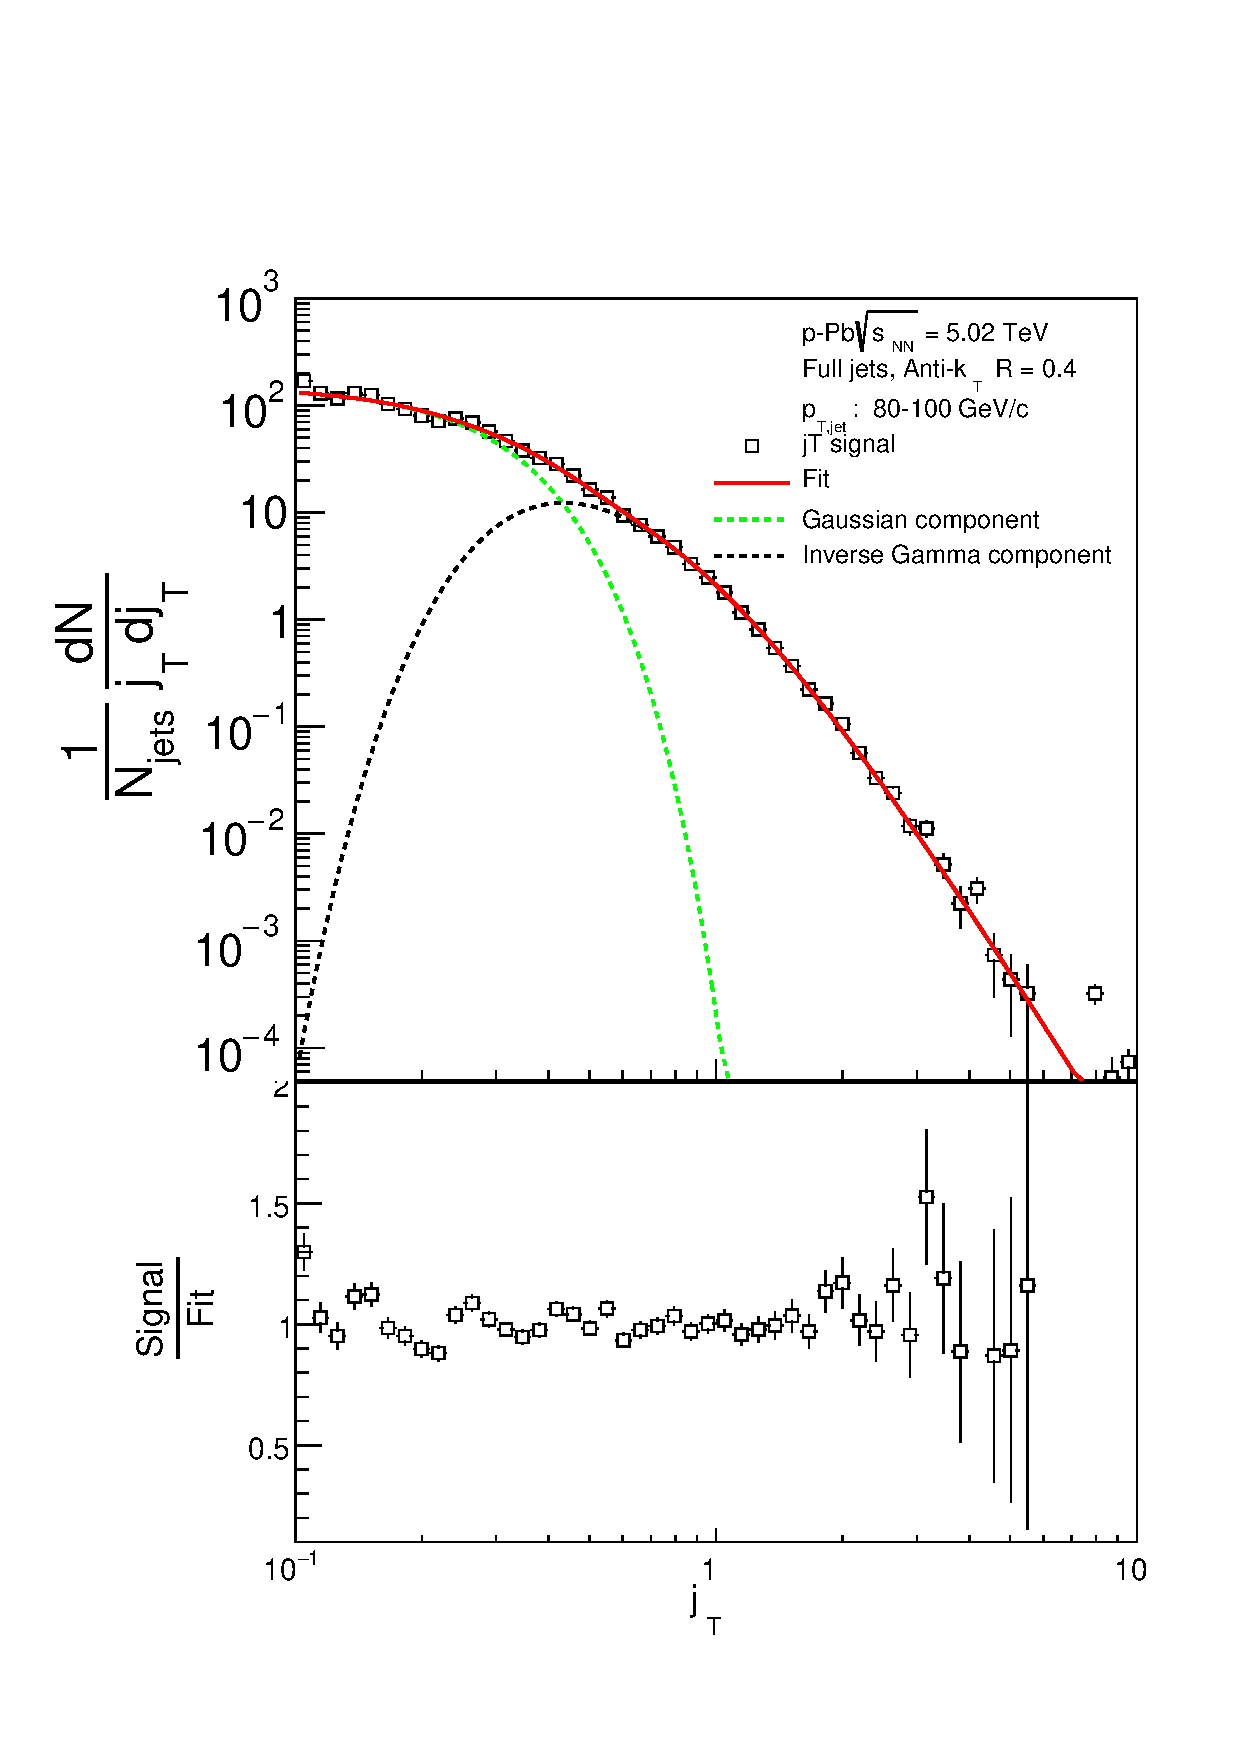
\includegraphics[width=0.95\textwidth]{results/JetConejTSignalFit/JetConejTSignalFitNFin00JetPt06randomBgBayes}
\end{subfigure}
\begin{subfigure}{0.24\textwidth}
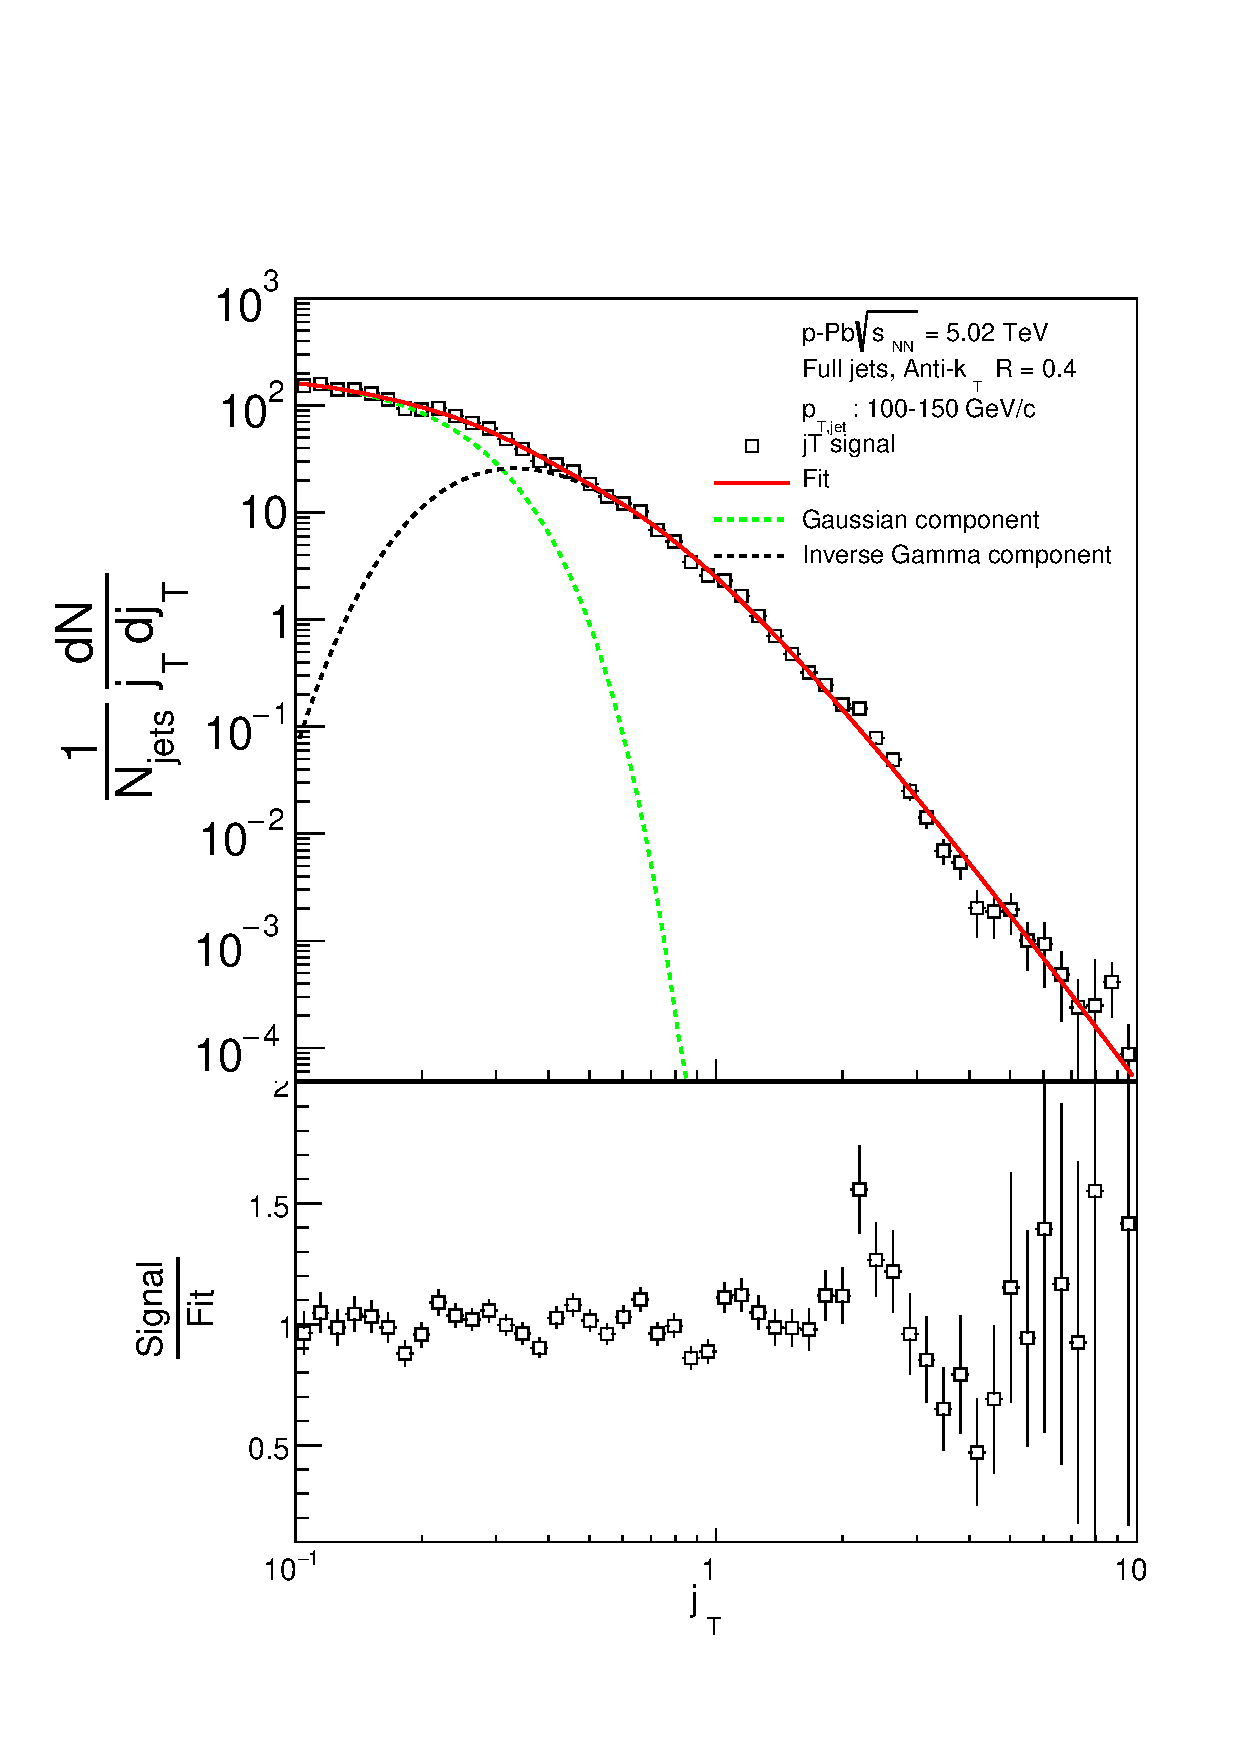
\includegraphics[width=0.95\textwidth]{results/JetConejTSignalFit/JetConejTSignalFitNFin00JetPt07randomBgBayes}
\end{subfigure}
\caption{$j_T$ signal with random bacgkround subtraction fits in different jet $p_T$ bins}
\label{fig:fitsrandombg}
\end{figure}

\subsection{Unfolding}
Unfolding is performed using both SVD and Bayesian unfolding. Difference between the methods is taken as the systematic error. Since SVD unfolding does not have a 2 dimensional options, the unfolding is done bin by bin. The resulting distributions after SVD unfolding and background subtraction with the perpendicular cone method are shown in fig \ref{fig:fitsSVD}. Resulting differences between the methods for different components are shown in figure \ref{fig:systunf}.

\begin{figure}
\centering
\begin{subfigure}{0.24\textwidth}
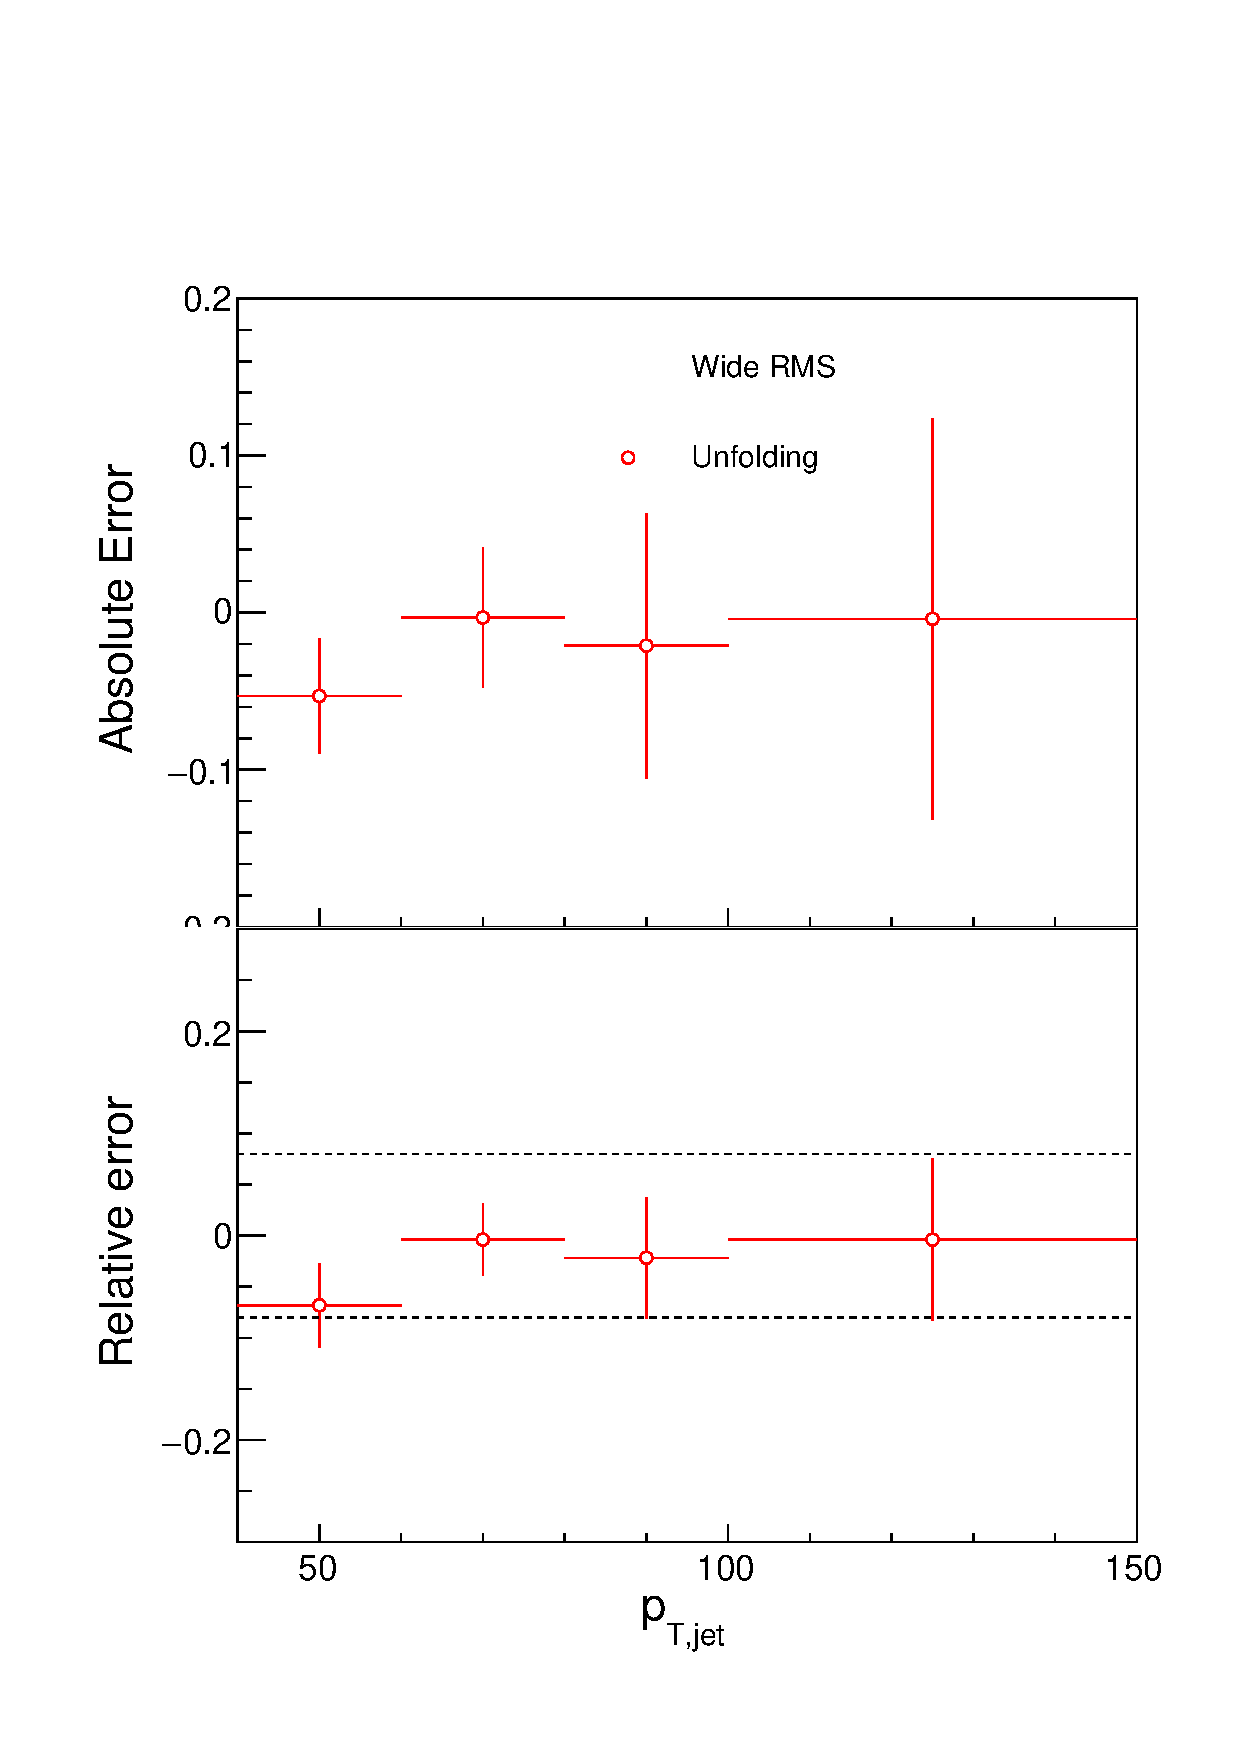
\includegraphics[width=0.95\textwidth]{results/SystematicErrors/SystematicErrorsGammaRMS_UnfNFin00JetPt08_linx_data}
\end{subfigure}
\begin{subfigure}{0.24\textwidth}
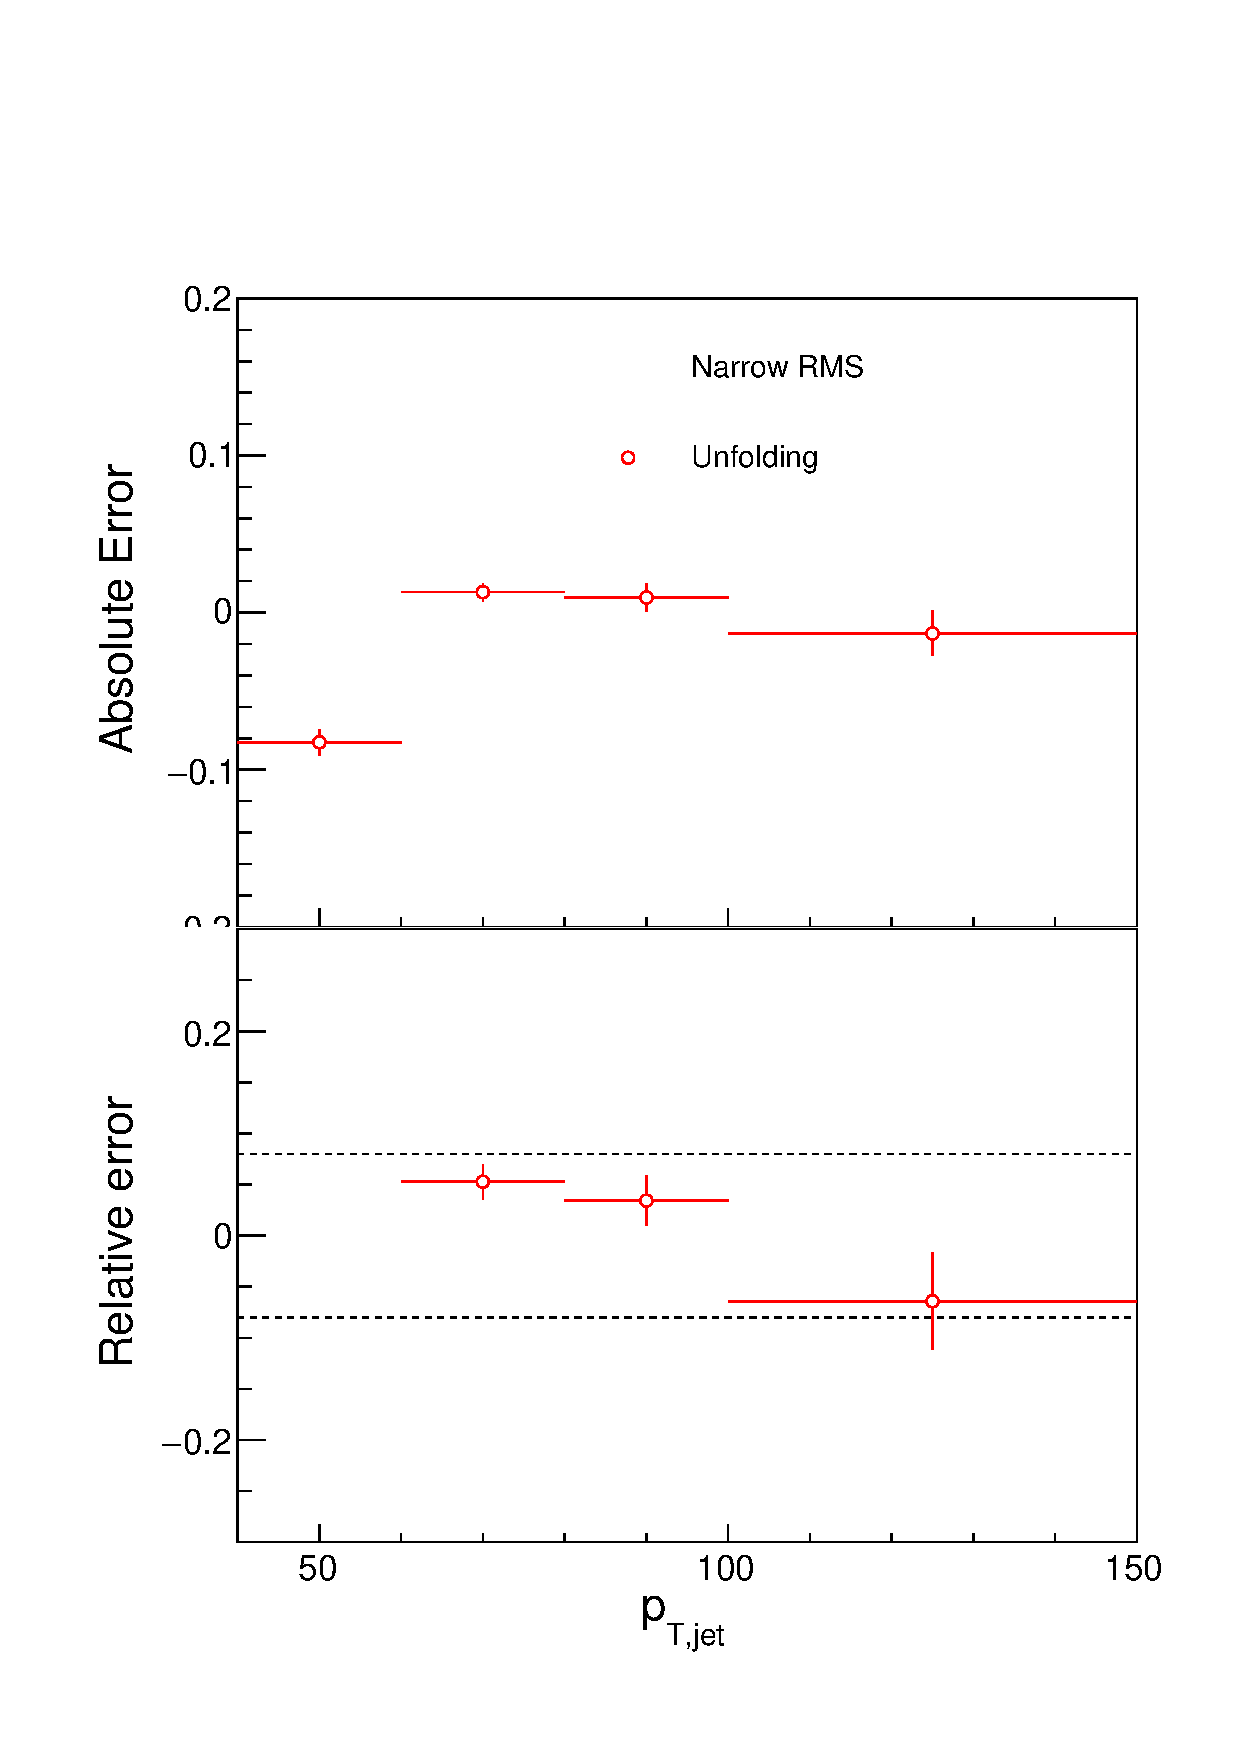
\includegraphics[width=0.95\textwidth]{results/SystematicErrors/SystematicErrorsGausRMS_UnfNFin00JetPt08_linx_data}
\end{subfigure}
\caption{Differences between Bayesian and SVD unfolding in the resulting RMS values}
\label{fig:systunf}
\end{figure}

\subsection{Tracking}

\subsection{Combining systematics}
Resulting systematic erros are shown in table \ref{tab:systematics}. Systematic errors are combined bin-by-bin in quadrature to get the total systematic errors.
\begin{table}[htb]
\centering
\caption{Summary of systematic errors}
\label{tab:systematics}
\begin{tabular}{ l | c | r }
  Systematic & Wide RMS & Narrow RMS \\
    \hline			
  Background & 5 \% & 9 \% \\
  Unfolding & 8 \% & 8 \% \\
  Total & 9 \% & 12\% \\
  \hline
  \end{tabular}
  \end{table}